\section{Induced Topologies} 

\subsection{Initial and Final Topologies} 

  We have seen some examples of how to create topologies. They can be created without any assumptions on the set, such as the discrete, indiscrete, and the cofinite topologies. More often, we want to consider how a certain structure like the order or a metric induces a topology. Now, we will consider how \textit{functions} can induce a topology. The uniqueness of such induced topologies is called the \textit{universal property}. 

  \begin{definition}[Initial Topology]
    Given a space $X$ and a family of topological spaces $\{Y_\alpha\}_{\alpha \in A}$ 
    \begin{equation}
      f_i : X \rightarrow (Y_\alpha, \T_\alpha)
    \end{equation} 
    the \textbf{initial topology} on $X$ is the coarsest topology $\T$ on $X$ s.t. that each 
    \begin{equation}
      f_i (X, \T) \rightarrow (Y_\alpha, \T_\alpha)
    \end{equation}
    is continuous. 
  \end{definition}

  \begin{definition}[Final Topology]
    Given a space $Y$ and a family of topological spaces $\{X_\alpha\}_{\alpha \in A}$ 
    \begin{equation}
      f: (X, \T_\alpha) \rightarrow Y
    \end{equation}
    the \textbf{final topology} on $Y$ is the finest topology $\T$ on $Y$ s.t. each 
    \begin{equation}
      f: (X, \T_\alpha) \rightarrow (Y, \T)
    \end{equation}
    is continuous. 
  \end{definition}

  Note that it makes sense to talk about the coarsest topology on the domain and the finest topology on the codomain. If it were the other way around, i.e. the finest topology on the domain, then the initial topology on $X$ would be the discrete topology, making every function defined on $X$ continuous. In the same logic, the coarsest topology on $Y$ would trivially be the trivial topology, making all $Y$-valued functions continuous. With these current definitions, if $\T_Y$ is too fine (e.g. if $\T_Y = 2^Y$), then the open sets of $\T_Y$ would be too fine and therefore would have a preimage that may not be open in $X$. 

\subsection{Subspace Topology} 

  The reason we want to do this is because we want to think of $Y$ as its own entity, independent of $X$. 

  \begin{definition}[Subspace Topology]
    Given topological space $X$ and subspace $Y \subset X$, the \textbf{subspace topology} on $Y$ is defined in the equivalent ways. 
    \begin{enumerate}
      \item It is the initial topology on the subspace $Y$ with respect to the inclusion map $\iota: Y \rightarrow X$. 
      \item It is the topology consisting of $X$-open sets intersection $Y$. 
      \begin{equation}
        \T_Y = \{(U \cap Y) \subset Y \mid U \in \T_X\}
      \end{equation}
    \end{enumerate}

    \begin{figure}[H]
      \centering
      \begin{subfigure}[b]{0.48\textwidth}
        \centering
        \begin{tikzpicture}
          % Draw the x and y axes in gray
          \draw[gray] (-3,0) -- (3,0);
          \draw[gray] (-1,-2) -- (-1,2);
          
          % Draw a blob (open set) with dotted borders
          \draw[dotted, thick] plot [smooth cycle, tension=0.8] coordinates {(-1,1) (0,1.5) (1.5,1) (2,-0.5) (1,-1.5) (-0.5,-0.8) (-1.5,-0.2)};
          
          % Label the open set
          \node at (0.0,0.8) {$U \in \mathscr{T}_{\mathbb{R}^2}$};
          
          % Draw a straight line passing through the blob with arrows on both ends
          \draw[-{Stealth[length=3mm]}, blue] (-2.5,-1.8) -- (2.5,1.8);
          
          % Label the line
          \node[anchor=north, blue] at (1.5,2) {$\ell \subset \mathbb{R}^2$};
          
          % Bold the portion where the line intersects the blob
          % Calculate or estimate intersection points
          \draw[thick, red] (-0.9,-0.65) -- (1.4, 1.0);
          
          % Label the intersection
          \node[red, anchor=south west] at (0,-0.7) {$V \in \mathscr{T}_\ell$};
          
          % Draw circles at the intersection points
          \draw[red] (-0.9,-0.65) circle (0.05);
          \draw[red] (1.4,1.0) circle (0.05);
        \end{tikzpicture}
        \caption{The subspace topology of a line $l$ in $\mathbb{R}^2$.}
        \label{fig:subspacer2}
      \end{subfigure}
      \hfill 
      \begin{subfigure}[b]{0.48\textwidth}
        \centering
        \tikzset{
          pattern size/.store in=\mcSize, 
          pattern size = 5pt,
          pattern thickness/.store in=\mcThickness, 
          pattern thickness = 0.3pt,
          pattern radius/.store in=\mcRadius, 
          pattern radius = 1pt}
          \makeatletter
          \pgfutil@ifundefined{pgf@pattern@name@_kou00hae2}{
          \pgfdeclarepatternformonly[\mcThickness,\mcSize]{_kou00hae2}
          {\pgfqpoint{0pt}{0pt}}
          {\pgfpoint{\mcSize+\mcThickness}{\mcSize+\mcThickness}}
          {\pgfpoint{\mcSize}{\mcSize}}
          {
          \pgfsetcolor{\tikz@pattern@color}
          \pgfsetlinewidth{\mcThickness}
          \pgfpathmoveto{\pgfqpoint{0pt}{0pt}}
          \pgfpathlineto{\pgfpoint{\mcSize+\mcThickness}{\mcSize+\mcThickness}}
          \pgfusepath{stroke}
        }}
        \makeatother
        \tikzset{every picture/.style={line width=0.75pt}}        
        \begin{tikzpicture}[x=0.75pt,y=0.75pt,yscale=-0.7,xscale=0.7]
          \draw  [color=blue,draw opacity=1][dash pattern={on 4.5pt off 4.5pt}] (291.17,116.36) .. controls (291.17,108.7) and (311.31,102.5) .. (336.17,102.5) .. controls (361.02,102.5) and (381.17,108.7) .. (381.17,116.36) .. controls (381.17,124.01) and (361.02,130.21) .. (336.17,130.21) .. controls (311.31,130.21) and (291.17,124.01) .. (291.17,116.36) -- cycle ;
          \draw    (272.32,35.59) .. controls (324.17,100.5) and (372.92,78.58) .. (470.17,20.5) ;
          \draw    (182.17,197.5) .. controls (273.66,272.15) and (386.17,172.5) .. (446.17,203.5) ;
          \draw    (272.32,35.59) .. controls (245.26,184.08) and (242.74,206.43) .. (182.17,197.5) ;
          \draw    (470.17,20.5) .. controls (501.17,119.5) and (470.17,190.5) .. (446.17,203.5) ;
          \draw  [color=blue,draw opacity=1][dash pattern={on 4.5pt off 4.5pt}] (285.17,138.12) .. controls (285.22,109.89) and (308.14,87.05) .. (336.37,87.1) .. controls (364.6,87.15) and (387.45,110.07) .. (387.4,138.3) .. controls (387.35,166.53) and (364.42,189.37) .. (336.19,189.33) .. controls (307.96,189.28) and (285.12,166.35) .. (285.17,138.12) -- cycle ;
          \draw  [color=red,draw opacity=1][pattern=_kou00hae2,pattern size=6pt,pattern thickness=0.75pt,pattern radius=0pt, pattern color=red][dash pattern={on 4.5pt off 4.5pt}] (337.41,141.34) .. controls (358.41,126.34) and (400.91,124.76) .. (380.91,144.76) .. controls (360.91,164.76) and (310.91,174.76) .. (290.91,144.76) .. controls (270.91,114.76) and (316.41,156.34) .. (337.41,141.34) -- cycle ;
          \draw  [color=blue,draw opacity=1][dash pattern={on 4.5pt off 4.5pt}] (302.17,173.86) .. controls (302.17,168.69) and (317.39,164.5) .. (336.17,164.5) .. controls (354.94,164.5) and (370.17,168.69) .. (370.17,173.86) .. controls (370.17,179.02) and (354.94,183.21) .. (336.17,183.21) .. controls (317.39,183.21) and (302.17,179.02) .. (302.17,173.86) -- cycle ;

          \node at (225,100) {$S \subset \mathbb{R}^3$};
          \node[blue] at (430,138) {$U \in \mathscr{T}_{\mathbb{R}^3}$};
          \node[red] at (240,150) {$V \in \mathscr{T}_{S}$};
        \end{tikzpicture}
        \caption{The subspace topology of a surface $\mathcal{L}$ in $\mathbb{R}^3$.}
        \label{fig:subspacer3}
      \end{subfigure}
      \caption{Visual of subspace topology.}
      \label{fig:subspace_topology}
    \end{figure}
  \end{definition} 
  \begin{proof}
    We prove the properties. 
    \begin{enumerate}
      \item \textit{Trivial}. We see that $\emptyset = \emptyset \cap Y$ and $Y = X \cap Y$. 
      \item \textit{Stability under Union}. Suppose $\{V_\alpha\}_{\alpha \in A}$ are setes that are open in $Y$. Then for each $\alpha$ there exists an open set $U_\alpha \subset X$ that is open in $X$. Therefore, 
      \begin{align}
        \bigcup_{\alpha \in A} V_\alpha & = \bigcup_{\alpha \in A} (U_\alpha \cap Y) \\ 
                                        & = Y \cap \bigg( \bigcup_{\alpha \in A} U_\alpha \bigg)
      \end{align}
      where $\cup_\alpha U_\alpha$ is open in $X$, and therefore we shown that there exists such an open set. 

      \item \textit{Stability under Finite Intersection}. Suppose $\{V_i\}_{i = 1}^n$ are open in $Y$. Then we can do the same thing. 
    \end{enumerate}
  \end{proof} 

  Furthermore, we can immediately retrieve the basis of the subspace topology. 

  \begin{theorem}[Induced Basis of Subspace Topologies]
    If $\B$ is a basis for the topology of $X$, then 
    \begin{equation}
      \B_Y \coloneqq \{B \cap Y \mid B \in \B \} 
    \end{equation}
    is a basis for the subspace topology of $Y$. 
  \end{theorem}
  \begin{proof}
    
  \end{proof}

  Since the subspace is so natural to consider, we will by default imply that if $X$ is a topological space and $Z \subset X$, $Z$ is endowed the subspace topology. 

  \begin{lemma}[Restrictions and Injections are Continuous]
    The results immediately follow: 
    \begin{enumerate}
      \item Given $f: X \rightarrow Y$ and $Z \subset X$, $f|_{Z} : Z \rightarrow Y$ is continuous. 
      \item Given $X$ and $Z \subset X$, the canonical injection $\iota: Z \rightarrow X$ is continuous. 
    \end{enumerate}
  \end{lemma}
  \begin{proof}
    Listed. 
    \begin{enumerate}
      \item Let us take an open set $U$ in $Y$. Then it is of the form $V \cap Y$ for some $V$ open in $X$. Therefore taking the preimage gives 
      \begin{equation}
        f|_{Z}^{-1} (U) = f^{-1} (U) = f^{-1} (V \cap Y) = f^{-1} (V) \cap f^{-1} (Y) = f^{-1} (V) \cap Z
      \end{equation}
      where $f^{-1} (V)$ is open by continuity of $f$, and so the intersection is open. 

      \item This is true by definition. 
    \end{enumerate}
  \end{proof}

  Given these results, one may wonder whether---just like how we restricted a continuous function to a smaller continuous function---we can ``extend'' a function to a larger function. However, this is not always true. 

  \begin{example}[Combining Continuous Functions May not be Continuous]
    Let us take $\mathbb{R}$ and divide it into $\mathbb{Q}$ and $(\mathbb{R} \setminus \mathbb{Q}) \setminus \{0\}$. Then let us define 
    \begin{align}
      f: \mathbb{Q} \rightarrow \mathbb{R} & f(x) = 0 \\ 
      g: (\mathbb{R} \setminus \mathbb{Q}) \setminus \{0\} \rightarrow \mathbb{R} & g(x) = x
    \end{align}
    Then $f$ and $g$ are trivially continuous, but taking the function 
    \begin{equation}
      h(x) \coloneqq \begin{cases} 
        f(x) = 0 & \text{ if } x \in \mathbb{Q} \\ 
        g(x) = x & \text{ if } x \not\in \mathbb{Q}
      \end{cases}
    \end{equation}
    which is not continuous.\footnote{Inspired from \href{https://math.stackexchange.com/questions/4034361/any-counter-example-of-pasting-lemma}{here}. }
  \end{example} 

  But not all hope is lost. It does turn out that under certain conditions, we can in fact construct such continuous functions. 

  \begin{lemma}[Pasting Lemma, Gluing Lemma]
    Let $X = A \cup B$, where $A, B$ are closed in $X$. Let $f: A \longrightarrow Y$ and $g: B \longrightarrow Y$ be continuous. If 
    \begin{equation}
      f(x) = g(x) \text{ for all } x \in A \cap B
    \end{equation}
    Then $f$ and $g$ can be combined to form a continuous function $h: X \longrightarrow Y$, defined
    \begin{equation}
      h(x) \equiv \begin{cases}
        f(x) & x \in A \setminus B \\
        f(x) \text{ or } g(x) & x \in A \cap B \\
        g(x) & x \in B \setminus A
      \end{cases}
    \end{equation}

    \begin{figure}[H]
      \centering 
      \begin{tikzpicture}[
        scale=1.2,
        set/.style={draw, thick},
        mapping/.style={->, thick},
        dashed mapping/.style={->, thick, dashed}
      ]
        % Set A with red north west lines pattern (smooth, asymmetric blob shape, vertically elongated)
        \begin{scope}
            \clip (-0.5,1.8) .. controls (-1.2,2.25) and (-2,1.8) .. 
                  (-2.3,0.6) .. controls (-2.5,-0.45) and (-1.8,-1.35) .. 
                  (-1,-1.05) .. controls (-0.2,-0.75) and (0.8,-0.3) .. 
                  (1.5,0.45) .. controls (2,1.2) and (1.5,2.1) .. 
                  (0.7,2.25) .. controls (0,2.3) and (-0.5,1.8) .. 
                  (-0.5,1.8) -- cycle;
            \fill[pattern=north west lines, pattern color=red!70] (-3,-3) rectangle (3,3);
        \end{scope}
        \draw[set] (-0.5,1.8) .. controls (-1.2,2.25) and (-2,1.8) .. 
                  (-2.3,0.6) .. controls (-2.5,-0.45) and (-1.8,-1.35) .. 
                  (-1,-1.05) .. controls (-0.2,-0.75) and (0.8,-0.3) .. 
                  (1.5,0.45) .. controls (2,1.2) and (1.5,2.1) .. 
                  (0.7,2.25) .. controls (0,2.3) and (-0.5,1.8) .. 
                  (-0.5,1.8) -- cycle;
        \node at (-1,0.75) {$A$};
        
        % Set B with blue north east lines pattern (asymmetric blob shape, vertically elongated)
        \begin{scope}
            \clip (-0.5,-1.95) .. controls (-1.8,-2.25) and (-2.5,-1.2) .. 
                  (-1.6,0) .. controls (-0.8,0.9) and (0.2,1.2) .. 
                  (1,0.75) .. controls (1.8,0.3) and (2.2,-0.45) .. 
                  (1.7,-1.5) .. controls (1,-2.25) and (0.3,-1.8) .. 
                  (-0.5,-1.95) -- cycle;
            \fill[pattern=north east lines, pattern color=blue!70] (-3,-3) rectangle (3,3);
        \end{scope}
        \draw[set] (-0.5,-1.95) .. controls (-1.8,-2.25) and (-2.5,-1.2) .. 
                  (-1.6,0) .. controls (-0.8,0.9) and (0.2,1.2) .. 
                  (1,0.75) .. controls (1.8,0.3) and (2.2,-0.45) .. 
                  (1.7,-1.5) .. controls (1,-2.25) and (0.3,-1.8) .. 
                  (-0.5,-1.95) -- cycle;
        \node at (1.2,-1.2) {$B$};
        
        % Add the intersection label
        \node at (0,0) {$A \cap B$};
        
        % Draw |___| shaped arrow at the bottom
        \draw[mapping] (0,-2.5) -- (0,-3) -- (5.3,-3) -- (5.3,-2.5) node[midway, left] {$h$};
        
        % Rectangle around right side (set Y)
        \draw[set] (3.8,-2) rectangle (6.8,2);
        \node at (6.4,-1.7) {$Y$};
        
        % Set f(A) on right with red north west lines pattern
        \begin{scope}
            \clip (5,1.5) .. controls (4.3,1.8) and (4,1.2) .. 
                  (4.2,0.5) .. controls (4.5,-0.3) and (5,-0.6) .. 
                  (5.8,-0.2) .. controls (6.3,0.2) and (6.5,0.8) .. 
                  (6.2,1.3) .. controls (5.8,1.7) and (5.5,1.3) .. 
                  (5,1.5) -- cycle;
            \fill[pattern=north west lines, pattern color=red!70] (3.5,-1) rectangle (7,2);
        \end{scope}
        \draw[set] (5,1.5) .. controls (4.3,1.8) and (4,1.2) .. 
                  (4.2,0.5) .. controls (4.5,-0.3) and (5,-0.6) .. 
                  (5.8,-0.2) .. controls (6.3,0.2) and (6.5,0.8) .. 
                  (6.2,1.3) .. controls (5.8,1.7) and (5.5,1.3) .. 
                  (5,1.5) -- cycle;
        \node at (5.3,0.5) {$f(A)$};
        
        % Set g(B) on right with blue north east lines pattern
        \begin{scope}
            \clip (5,-1.2) .. controls (4.2,-1.5) and (4,-0.8) .. 
                  (4.3,-0.3) .. controls (4.7,0.3) and (5.3,0.5) .. 
                  (5.9,0.1) .. controls (6.5,-0.3) and (6.4,-1) .. 
                  (5.8,-1.4) .. controls (5.4,-1.6) and (5,-1) .. 
                  (5,-1.2) -- cycle;
            \fill[pattern=north east lines, pattern color=blue!70] (3.5,-2) rectangle (7,1);
        \end{scope}
        \draw[set] (5,-1.2) .. controls (4.2,-1.5) and (4,-0.8) .. 
                  (4.3,-0.3) .. controls (4.7,0.3) and (5.3,0.5) .. 
                  (5.9,0.1) .. controls (6.5,-0.3) and (6.4,-1) .. 
                  (5.8,-1.4) .. controls (5.4,-1.6) and (5,-1) .. 
                  (5,-1.2) -- cycle;
        \node at (5.3,-0.8) {$g(B)$};
        
        % Dotted arrows for direct mappings
        \draw[dashed mapping] (-0.5,1) to[out=20, in=160] node[midway, above] {$f$} (4.3,1);
        \draw[dashed mapping] (-0.3,-1.5) to[out=-20, in=200] node[midway, below] {$g$} (4.3,-1);
        \draw[dashed mapping] (0,0) to[out=0, in=180] node[midway, above] {$f$ or $g$} (4.8,0);
      \end{tikzpicture}
      \caption{Visual of the pasting lemma.} 
      \label{fig:gluing_lemma}
    \end{figure}
  \end{lemma}

  Consider any set $U \subset Y$. Note that if $U$ is an open set in $X$ that happens to be contained in $Y$, then we can set $U = U \cap Y$, so $U$ is open in $Y$. However, we have seen that being open in $Y$ does not necessarily imply that it is open in $X$. 

  \begin{example}[Non-Open Sets may be Open in Subspace]
    Let $X = \mathbb{R}$ with the Euclidean topology and let $Y = [0, 1]$. 
    \begin{enumerate}
      \item $[0, 1]$ is open in $Y$ but not open in $X$. 
      \item Intervals of the form $(a, 1]$ and $[0, b)$ are open in $Y$ but not open (nor closed) in $X$. 
    \end{enumerate}
  \end{example} 

  \begin{example}[Singleton Sets in Subspace Topologies]
    Consider $X = \mathbb{R}$ with the lower limit topology with $Y = [0, 1]$. The following 
    \begin{enumerate}
      \item $[1/2, 1] = Y \cap [1/2, 2)$, and 
      \item $\{1\} = Y \cap [1, 2)$
    \end{enumerate}
    are open in the subspace topology. It turns out that $\{1\}$ is the only singleton set open in $Y$. 
  \end{example}

  Let's go through a few examples. 

  \begin{example}[Closed Unit Interval in $\mathbb{R}$]
    The basis for the subspace topology of $[0, 1] \subset \mathbb{R}$ with the Euclidean topology consists of the intervals 
    \begin{enumerate}
      \item $(a, b)$ where $0 \leq a < b \leq 1$. 
      \item $[0, b)$ where $0 < b \leq 1$. 
      \item $(a, 1]$ where $0 \leq a < 1$. 
    \end{enumerate}
  \end{example} 

  \begin{example}[Unit Sphere in $\mathbb{R}^n$] 
    Let $S^n \subset \mathbb{R}^{n+1}$ be the unit \textbf{n-sphere} defined $S^n \coloneqq \{x \in \mathbb{R}^{n+1} \mid ||x||^2 = 1 \}$. When thinking about $S^n$ as a space itself, we use the subspace topology coming from the standard topology of $\mathbb{R}^n$. 
  \end{example}

  \begin{example}[$S^1 \subset \mathbb{R}^2$]
    Let's focus on $n = 1$. For $a < b$, let 
    \begin{equation}
      A_{a, b} = \{ (\cos{t}, \sin{t}) \mid a < t < b \}
    \end{equation} 
    Then, we can see that
    \begin{enumerate}
      \item if $b - a > 2 \pi$, then $A_{a, b} = S^1$. 
      \item If $b - a \leq 2 \pi$, then $A_{a, b}$ is an ``open arc'' from $(\cos{a}, \sin{a})$ to $(\cos{b}, \sin{b})$.  
    \end{enumerate} 

    Given that we have an equivalence class defined 
    \begin{equation}
      A_{a, b} \sim A_{a + 2 \pi k, b + 2 \pi k} \text{ for all } k \in \mathbb{Z}
    \end{equation} 
    We claim that $\{A_{a, b}\}$ is a basis for the subspace topology of $S^1$. We can see that the open arc covering the top right quadrant in $\mathbb{R}^2$ is 
    \begin{equation}
      S^1 \cap (0, 1)^2 = S^1 \cap B_\infty \big( (\frac{1}{2}, \frac{1}{2}), \frac{1}{2} \big)
    \end{equation}
  \end{example}

  Now let's focus more on metric spaces. Note that if we want to construct topologies of subspaces of metric spaces, there are two ways to do it. It would be quite bad if these resulted in different topologies, but fortunately we have the following theorem. 

  \begin{theorem}[Topologies on Subspaces of Metric Spaces Coincide]
    Let $(X, d_X)$ be a metric space, with $Y \subset X$. There are 2 ways we can define a topology on $Y$. 
    \begin{enumerate}
      \item Take the metric topology $\T_X$ on $X$, and then take the subspace topology on $Y$. 
      \item Induce a metric $d_Y = d_{X | Y}$ on $Y$ which is a restriction of $d_X$ to $Y$, and then take the metric topology of it. 
    \end{enumerate}
    We claim that these two constructions give the same topology, as shown in the commutative diagram. 

    \begin{figure}[H]
      \centering 
      \begin{tikzcd}
        d_X \arrow[r] \arrow[d] & d_Y \arrow[d] \\
        \T_X \arrow[r] & \T_Y 
      \end{tikzcd}
      \caption{} 
      \label{fig:same_construction}
    \end{figure}
  \end{theorem}
  \begin{proof}
    The basis for the subspace topology on $Y$ is 
    \begin{equation}
      \B_1 = \{B_{d_X} (x, r) \cap Y \mid x \in X, r > 0 \}
    \end{equation} 
    and the basis for the (induced) metric topology on $Y$ is 
    \begin{equation}
      \B_2 = \{B_{d_Y} (y, r) \cap Y \mid y \in Y, r > 0 \} = \{B_{d_X} (y, r) \cap Y \mid y \in Y, r > 0 \}
    \end{equation} 
    It is immediate that $\B_2 \subset \B_1$ since it goes over all $x \in X$ rather than $y \in Y$. To see why $\B_1 \subset \B_2$, TBD. 
  \end{proof}

  \begin{theorem}[Closures in Subspace Topologies]
    Let $A \subset Y \subset X$. Let $\bar{A}$ denote the closure of $A$ in $X$. Then, the closure of $A$ in $Y$ equals $\bar{A} \cap Y$. 
  \end{theorem}

\subsection{Box Topology} 

  There are multiple ways to define the box and product topologies, but their construction with basis elements is most simple. 

  \begin{definition}[Box Topology]
    Given a family of topological spaces $\{(X_\alpha, \T_\alpha)\}_{\alpha \in A}$, the \textbf{box topology} on the space $\prod_{\alpha \in A} X_\alpha$ is the topology generated by the basis 
    \begin{equation}
      \mathscr{B} = \bigg\{ \prod_{\alpha \in A} U_\alpha \mid U_\alpha \in \T_\alpha \bigg\}
    \end{equation}

    \begin{figure}[H]
      \centering 
      \begin{tikzpicture}
        \draw[<->] (-1,0)--(6,0);
        \draw[<->] (0,-1)--(0,4);
        \draw[dashed] (1,1)--(1,3)--(4,3)--(4,1)--(1,1);
        \node[below] at (6,0) {$\mathbb{R}$};
        \node[left] at (0,4) {$\mathbb{R}$};
        \node[below] at (1,-0.3) {$a$};
        \node[below] at (4,-0.3) {$b$};
        \node[left] at (-0.3,1) {$c$};
        \node[left] at (-0.3,3) {$d$};
        \node[rotate=90] at (0,1) {$($};
        \node[rotate=-90] at (0,3) {$($};
        \node at (1,0) {$($};
        \node at (4,0) {$)$};
      \end{tikzpicture}
      \caption{We can visualize the elements of the box topology with the product space $\mathbb{R}^2 = \mathbb{R} \times \mathbb{R}$, where each $\mathbb{R}$ has an open ball topology. From the visual below, we can see why this is called the "box" topology. }
      \label{fig:box_topology}
    \end{figure}
  \end{definition}
  \begin{proof}
    It is easy to prove that the box topology indeed satisfies the 3 properties of topologies in general. 
  \end{proof}

\subsection{Product Topology}

  While the box topology may seem quite "intuitive" for the first learner, the box topology however, has serious limitations when extending to infinite Cartesian products of spaces. To motivate the product topology, let's try to ``reverse engineer'' a topology on $X \times Y$ such that the projection mappings $\pi_1: X \times Y \rightarrow X$ is always continuous. We want 
  \begin{enumerate}
    \item $U \times Y$ to be open for $U \subset X$ open. 
    \item $X \times V$ to be open for $V \subset Y$ open. 
  \end{enumerate}
  This implies that $(U \times Y) \cap (X \times V) = U \times V$ should be open. This is how we will define the product topology. The main difference between the construction of open sets in the box topology vs the product topology is that the box topology merely describes open sets as direct products of open sets from each coordinate space while the construction of the product topology is completely dependent on the projection mappings $\pi_\beta: \prod_{\alpha \in I} X_\alpha \rightarrow X_\beta$ to be continuous (and nothing more) so that (by definition) the preimages of open sets in $X_\beta$ under $\pi_\beta$ are open sets in $\prod X_\alpha$. Therefore, the construction of the continuous $\pi_\beta$'s canonically constructs a basis of open sets in $\prod X_\alpha$. 

  \begin{definition}[Product Topology] 
    Given a family of topological spaces $\{(X_\alpha, \T_\alpha)\}_{\alpha \in A}$, the \textbf{product topology} on the space $\prod_{\alpha \in A} X_\alpha$ is defined in the following equivalent ways. 
    \begin{enumerate}
      \item It is the initial topology on the product space wrt the family of projections $p_\alpha: \prod_{\alpha \in A} X_\alpha \rightarrow X_\alpha$. 

      \item It is the topology generated by the basis of elements 
      \begin{equation}
        \prod_\alpha U_\alpha 
      \end{equation}
      where $U_\alpha$ is a proper open subset for at most finitely many $\alpha$'s, and $U_\alpha = X_\alpha$ for all other $\alpha$. 
    \end{enumerate}

    \begin{figure}[H]
      \centering 
      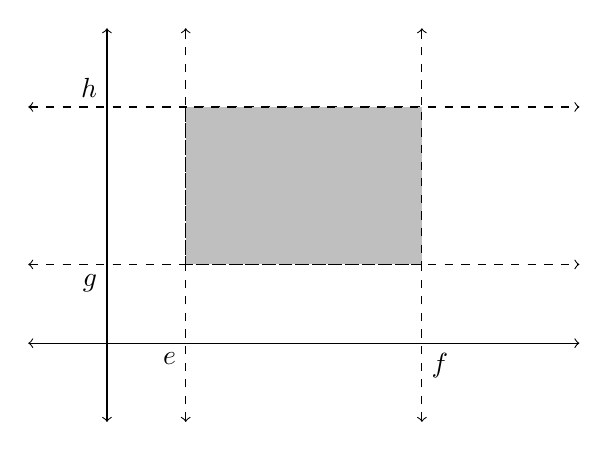
\begin{tikzpicture}
        \draw[<->] (-1,0)--(6,0);
        \draw[<->] (0,-1)--(0,4);
        \draw[<->, dashed] (-1,1)--(6,1);
        \draw[<->, dashed] (-1,3)--(6,3);
        \draw[<->, dashed] (1,-1)--(1,4);
        \draw[<->, dashed] (4,-1)--(4,4);
        \node [below left] at (1,0) {$e$};
        \node [below right] at (4,0) {$f$};
        \node [above left] at (0,3) {$h$};
        \node [below left] at (0,1) {$g$};
        \draw[dashed, fill=lightgray] (1,1) rectangle (4,3);
      \end{tikzpicture}
      \caption{Visually, we can interpret each $\mathscr{S} (U_\beta)$ as a "strip" in the total product space. For example in $\mathbb{R}^2$, there are two "strips" $(e, f) \times \mathbb{R}$ and $\mathbb{R} \times (g, h)$ that intersect. Note that each strip is the preimage of the projection mapping. }
      \label{fig:product_topology}
    \end{figure}
  \end{definition}

  We can deduce some conclusions comparing these topologies. First, the product and box topologies are precisely the same if we work in finite Cartesian products of spaces, since any element of the box topology (left hand side) can be expressed as a finite intersection of some open sets (in the right hand side). That is, if $\text{card}\,I < \infty$, then 
  \begin{equation}
    \prod_{\alpha \in I} U_i = \bigcap_{\alpha \in I} \big\{ \prod_{\gamma \in I} W_\gamma \mid W_\gamma = U_\gamma \text{ if } \gamma = \alpha, \, W_\gamma = X_\gamma \text{ if } \gamma \neq \alpha\big\}
  \end{equation}
  Secondly, we can see that the box topology is finer than the product topology (strictly finer if working in infinite product spaces). 

  \begin{example}
    The set $(0,1)^\mathbb{N} \subset \mathbb{R}^\mathbb{N}$ is clearly open in the box topology, but it is considered "too tight" to be in the product topology. However, 
    \begin{equation}
      (0,1) \times \mathbb{R} \times \mathbb{R} \times \ldots
    \end{equation}
    is open in the product topology since only one (a finite amount) of the factors is not the whole space. 
  \end{example}

  The following theorem reveals why the product topology is superior than the box topology in product spaces. 

  \begin{theorem}[Continuity of Functions Mapped to Product Topology]
    Given the function 
    \begin{equation}
      f: A \rightarrow \prod_{\alpha \in I} X_\alpha, \; f(a) \equiv \big( f_\alpha (a) \big)_{\alpha \in I}
    \end{equation}
    with its component functions $f_\alpha: A \rightarrow X_\alpha$. Let $\prod X_\alpha$ have the product topology. Then the function $f$ is continuous if and only if each function $f_\alpha$ is continuous. 
  \end{theorem}
  \begin{proof}
    We prove both directions. Let $\pi_\beta$ be the projection of this product onto the $\beta$th component space. By construction $\pi_\beta$ is continuous $\implies \pi_\beta^{-1} (U_\beta)$ is a basis element of the product topology of $\prod X_\alpha$. 
    \begin{enumerate}
      \item $(\rightarrow)$ $f$ is continuous, so $f_\beta \equiv \pi_\beta \circ f$, as the composition of continuous functions, is also continuous. 
      \item $(\leftarrow)$ Assume that each $f_\beta$ is continuous. Let there be an open set $U_\beta \subset X_\beta$. Then, the canonical open set $\pi_\beta^{-1}$ in the product space $\prod X_\alpha$ is also open. Now, the preimage of $\pi_\beta^{-1} (U_\beta)$ under $f$ is 
      \begin{align*}
        f^{-1} \big( \pi_\beta^{-1} (U_\beta)\big) & = (f^{-1} \circ \pi_\beta^{-1})(U_\beta) \\
        & = (\pi_\beta \circ f)^{-1} (U_\beta) \\
        & = f_\beta^{-1} (U_\beta)
      \end{align*}
      Since $f_\beta$ is already assumed to be continuous, $f_\beta^{-1} (U_\beta)$ is open in $A$. 
    \end{enumerate}
  \end{proof} 

  This theorem also works for the box topology only if we are working with finite product spaces. But in general, this theorem fails for the box topology. Consider the following example. 

  \begin{example}
    Let $\mathbb{R}^\omega$ be the countably infinite product of $\mathbb{R}$'s. Let us define the function 
    \begin{equation}
      f: \mathbb{R} \rightarrow \mathbb{R}^\omega
    \end{equation}
    with coordinate function defined $f_n (t) \equiv t$ for all $n \in \mathbb{N}$. Clearly, each $f_n$ is continuous. Given the box topology, we consider one basis element of $\mathbb{R}^\omega$
    \begin{equation}
      B = \prod_{i=1}^\infty (-\frac{1}{i}, \frac{1}{i})
    \end{equation}
    Assume that $f$ is continuous, that is $f^{-1}(B)$ is open in $\mathbb{R}$. Then, it would contain some finite interval $(-\delta, \delta)$ about $0$, meaning that $f\big( (-\delta, \delta)\big) \subset B$. This implies that for each $n \in \mathbb{N}$, 
    \begin{equation}
      f_n \big( (-\delta, \delta) \big) = (-\delta, \delta) \subset \Big( -\frac{1}{n}, \frac{1}{n} \Big)
    \end{equation}
    which contradicts the fact that $B$ is open, since the interval $(-1/n, 1/n)$ converges onto a point $0$. 
  \end{example}

  However, there is no useful criterion for the continuity of a mapping $f: X \times Y \longrightarrow A$ even if we have the product topology on $X \times Y$. One might conjecture that this $f$ is continuous if it is continuous in each variable separately, but this is in fact not true. 

  \begin{theorem}[Topologies on Products of Metric Spaces Coincide]
    Given a metric space
  \end{theorem}

  \begin{corollary}
    The Euclidean topology on $\mathbb{R}^n$ is equivalent to the product topology of the Euclidean topologies on $\mathbb{R}$. 
  \end{corollary} 

  \begin{theorem}[Subspace of Products and Products of Subspaces are Equivalent]
    If $A \subset X$ and $B \subset Y$, then the following topologies are equivalent. 
    \begin{enumerate}
      \item The subspace topology on the product topology of $X \times Y$. 
      \item The product topology on the subspace topologies of $A, B$. 
    \end{enumerate}
  \end{theorem}

  \begin{example}[Sorgenfrey Plane]
    The Cartesian product of two real lines with the lower limit topology is called the \textbf{Sorgenfrey plane}. 
    \begin{equation}
      \mathbb{R}_\ell \times \mathbb{R}_\ell
    \end{equation}
  \end{example}

  \begin{lemma}
    The addition, subtraction, and multiplication operations are continuous functions from $\mathbb{R} \times \mathbb{R} \longrightarrow \mathbb{R}$, and the quotient operation is a continuous function from $\mathbb{R} \times (\mathbb{R} \setminus \{0\}) \longrightarrow \mathbb{R}$. 
  \end{lemma}
  \begin{proof}
    Standard $\epsilon-\delta$ proof. 
  \end{proof}

  Now that we have defined what it means for binary operations to be continuous, we can talk about \textit{topological algebra}, which is the study of algebraic structures such that their algebraic operations and inverses are continuous. One important such concept is a \textit{topological group}, which will be mentioned later. 

\subsection{Quotient Topologies} 

  We have established natural topologies on sets that are constructed from other sets, namely by subsets and Cartesian products. Another way to construct a set is by taking an \hyperref[set-partition]{equivalence relation}, which partitions the set into its equivalence classes. The method in which we construct such a topology on this quotient space, called the \textit{quotient topology}, is slightly less straightforward.  

  \subsubsection{Quotient Maps}

    \begin{definition}[Quotient Map]
      A function $p: X \rightarrow Y$ is said to be a \textbf{quotient map} if it is surjective and 
      \begin{equation}
        U \text{ is open in } Y \iff p^{-1}(U) \text{ is open in } X
      \end{equation} 
      Note that we could have also replaced open with closed sets and the definitions are equivalent. 
    \end{definition}

    \begin{definition}[Saturation]
      A subset $S \subset X$ is \textbf{saturated} with respect to the surjective map $p: X \rightarrow Y$ if for every $p^{-1} (A)$ (where $A \subset Y$) that intersects $S$, $p^{-1}(A)$ is completely contained within $S$. That is, 
      \begin{equation}
        p^{-1} \big( p(S) \big) = S
      \end{equation}

      \begin{figure}[H]
        \centering 
        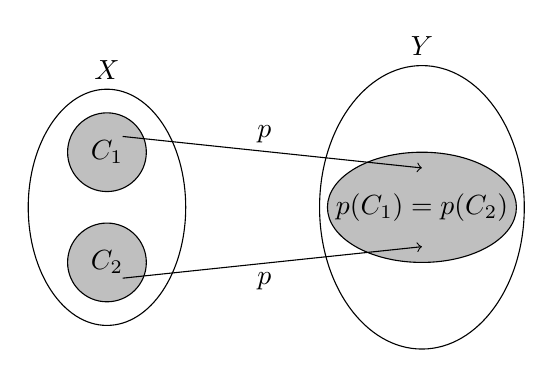
\begin{tikzpicture}
          \draw (0,0) ellipse (1 and 1.5);
          \draw[fill=lightgray] (0, 0.7) circle (0.5);
          \draw[fill=lightgray] (0, -0.7) circle (0.5);
          \node[above] at (0,1.5) {$X$};
          \draw (4,0) ellipse (1.3 and 1.8);
          \node[above] at (4,1.8) {$Y$};
          \draw[fill=lightgray] (4,0) ellipse (1.2 and 0.7);
          \node at (0, 0.7) {$C_1$};
          \node at (0,-0.7) {$C_2$};
          \node at (4,0) {$p(C_1) = p(C_2)$};
          \draw[->] (0.2,0.9)--(4,0.5);
          \draw[->] (0.2,-0.9)--(4,-0.5);
          \node[above] at (2, 0.7) {$p$};
          \node[below] at (2, -0.7) {$p$};
        \end{tikzpicture}
        \caption{We can see that $C_1$ and $C_2$ alone are not saturated, but $C_1 \cup C_2$ is saturated. Visually, for a given set $C \subset X$ to be saturated, there cannot be any points $q \not\in C$ such that $q \in p(C)$. }
        \label{fig:saturation}
      \end{figure}
    \end{definition}

    We now introduce an alternative, equivalent definition of quotient maps. 

    \begin{theorem}[Quotient Maps w.r.t. Mapping Saturated Sets]
      $p: X \rightarrow Y$ is a quotient map if and only if $p$ is continuous and $p$ maps saturated open sets of $X$ to open sets of $Y$ (or saturated closed sets of $X$ to closed sets of $Y$). 
    \end{theorem} 

    The first property is that quotient maps behave nicely under compositions. 

    \begin{theorem}[Composition of Quotient Maps]
      The composition of two quotient maps is a quotient map. 
    \end{theorem}
    \begin{proof}
      We immediately know that the composition of surjective maps are surjective and that of continuous maps are continuous. 
    \end{proof}

    However, they do not behave nicely under subspace or products. If $p: X \rightarrow Y$ is a quotient map and $A$ is a subspace of $X$, then the map $p^\prime: A \rightarrow p(A)$ obtained by restricting both the domain and codomain of $P$ need not be a quotient map. The product of two quotient maps is not necessarily a quotient map. That is, given $p: A \rightarrow B$ and $q: C \rightarrow D$ are quotient maps, the map 
    \begin{equation}
      p \times q: A \times C \rightarrow B \times D, \; (p \times q) (a \times c) \equiv p(a) \times q(c)
    \end{equation}
    is not necessarily a quotient map. 

    \begin{example}[Restriction of Quotient Maps are Not Quotient Maps]
      
    \end{example}

    \begin{example}[Products of Quotient Maps are Not Quotient Maps]
      
    \end{example}

    Additionally, quotient maps are clearly not homeomorphisms, so topological properties are not preserved. 

    \begin{example}[]
      
    \end{example}

    However, there is just one extra condition on a quotient map that will make it a homeomorphism.  

    \begin{lemma}[Bijective Quotient Maps]
      A quotient map that is injective (and hence bijective) is a homeomorphism. 
    \end{lemma} 

  \subsubsection{Open and Closed Maps}

    Open and closed functions map open/closed sets to open/closed sets, unlike continuous functions which take the preimage. However, they do are not natural and most maps are not open nor closed, so this is a pretty special condition. 

    \begin{definition}[Open, Closed Maps]
      A map $f: X \rightarrow Y$ is said to be 
      \begin{enumerate}
        \item \textbf{open} if it maps open sets of $X$ to open sets of $Y$. 
        \item \textbf{closed} if it maps open sets of $X$ to closed sets of $Y$. 
      \end{enumerate}
      Note that open and closed maps are completely independent. A map may be open, closed, neither, or both. 
    \end{definition}

    \begin{example}[Open but Not Closed]
      The projection $\pi_1: X \times Y \rightarrow X$ is an open map but but closed. Consider $\pi_1: \mathbb{R}^2 \rightarrow \mathbb{R}$ with $S = \{(x, y) \in \mathbb{R}^2 \mid xy = 1 \}$. Then $\pi_1 (S) = \mathbb{R} \setminus \{0\}$, which is not closed.\footnote{In open maps, the typical behavior is that points are ``copied,'' i.e. for projections, the preimage of $\pi_1^{-1} (x) = x \times Y$, where all $y \in Y$ are copied.}
    \end{example}

    \begin{example}[Closed but Not Open]
      $f: \mathbb{R} \rightarrow \mathbb{R}$ with $f(x) = x^2$ is closed but not open since $f(\mathbb{R}) = [0, +\infty)$ which is not open. 
    \end{example}

    Note that an open map or a closed map (with continuous and surjective) are trivially quotient maps. Since given a $U \subset Y$ with $f^{-1} (U)$ open, then by definition $U = f(f^{-1} (U))$ is open by definition. 

    \begin{theorem}[Open/Closed Maps are Stronger than Quotient Maps]
      If $p: X \rightarrow Y$ is a surjective, continuous map that is either open or closed (that is, maps open sets to open sets or closed sets to closed sets), then $p$ is a quotient map.\footnote{Note however, that the converse is not true; there exists quotient maps that are neither open nor closed. }
    \end{theorem} 

    \begin{example}[Quotient Maps that are Neither Open Nor Closed]
      
    \end{example}

  \subsubsection{Quotient Topology}

    Now that we have defined the quotient map, we are ready to define the quotient topology. 

    \begin{definition}[Quotient Topology]
      Let $p: (X, \T_X) \rightarrow Y$ be a surjective map.\footnote{A natural surjective map that we can construct is by taking an equivalence relation $\sim$ on $X$, setting $Y = X/\sim$, and taking $p: x \mapsto [x]$. Every surjective map can be thought of as a map induced by an equivalence relation, since we can set $x \sim x^\prime$ iff $f(x) = f(x^\prime)$, so these are equivalent.} Then, the \textbf{quotient topology} induced by $p$ is defined in the following equivalent ways. 
      \begin{enumerate}
        \item It is the final topology on the quotient set $X/\sim$ wrt the projection map $p$. 
        \item It is the topology of all subsets $U$ of $Y$ s.t. $p^{-1}$ is open in $X$. 
        \begin{equation}
          U \text{ open in } X/\sim \iff p^{-1} (U) \text{ saturated and open in } X
        \end{equation}
        \item It is the unique topology $\T_Y$ relative to which $p$ is a quotient map.\footnote{We claim that this topology exists and is unique.}
      \end{enumerate}
      The quotient set $X/\sim$ with its quotient topology is called the \textbf{quotient space}. 
    \end{definition}
    \begin{proof}
      The topology $\T_Y$ on $Y$ is defined by letting it consist of all subsets $U$ of $Y$ such that $p^{-1}(U)$ is open in $X$. This is indeed a topology since
      \begin{enumerate}
        \item $p^{-1} (\emptyset) = \emptyset$ and $p^{-1}(Y) = X$
        \item $p^{-1} \Big( \bigcup_{\alpha \in J} U_\alpha \Big) = \bigcup_{\alpha \in J} p^{-1} (U_\alpha)$
        \item $p^{-1} \Big( \bigcap_{i=1}^n U_i \Big) = \bigcap_{i=1}^n p^{-1} (U_i)$
      \end{enumerate}
    \end{proof}

    The intuition is the following. The topology on $X$ is fixed, and we must somehow find some topology on $Y$ that makes $p$ a quotient map. If we make $\T_Y$ too coarse, satisfiying continuity of $p$ is easy but it may not necessarily mean that $p^{-1}(U)$ open in $X$ implies $U$ open in $Y$. However, if we make $\T_Y$ too fine, then continuity may not be satisifed. The theorem states that there is a middle point---in fact exactly one topology---in which cases both directions are satisfied. 

    \begin{example}
      Let $p: (\mathbb{R}, \T_\mathbb{R}) \rightarrow \mathbb{R} / 2 \pi \mathbb{R}$. Then, the final topology of $\mathbb{R} / 2 \pi \mathbb{R}$ would be simply defined 
      \begin{equation}
        \T_{\mathbb{R} / 2 \pi \mathbb{R}} \equiv \{U \subset \mathbb{R} / 2\pi \mathbb{R} \mid U = p(O), O \in \T_\mathbb{R}\}
      \end{equation}
      That is, the quotient topology is merely the set of all images of open sets in $\mathbb{R}$ under $f$. However, if $\mathbb{R} / 2 \pi \mathbb{R}$ has the discrete topology $2^X$, then a single equivalence class, say $[0]$, will get mapped to the collection of points $\{2 \pi k \mid k \in \mathbb{Z}\}$, which is clearly not open in $\mathbb{R}$. Note that the final topology (or the quotient topology) is endowed onto the codomain in order to make $f$ continuous (or a quotient mapping). 
    \end{example}

    \begin{example}
      Let $X \equiv [0,1] \cap [2,3] \subset \mathbb{R}$ and $Y y \equiv [0,2] \subset \mathbb{R}$. Then, we define $p: X \rightarrow Y$ as 
      \begin{equation}
        p(x) \equiv \begin{cases} x & x \in [0,1] \\ x-1 & x \in [2,3] \end{cases}
      \end{equation}
      $p$ is continuous (under subspace topology of $X \subset \mathbb{R}$), surjective, and closed, meaning that it is a quotient map. However, it is not open, since the image of the open set $[0,1]$ of $X$ is $[0,1]$, which is not open in $Y$. 
    \end{example}

    \begin{example}[Finite Sets]
      Let $p: \mathbb{R} \rightarrow \{a, b, c\}$ be defined as 
      \begin{equation}
        p(x) \equiv \begin{cases} a & x > 0 \\ b & x < 0 \\ c & x = 0 \end{cases}
      \end{equation}
      Then, the quotient topology of $\{a, b, c\}$ consists of 
      \begin{equation}
        \emptyset, \{a\}, \{b\}, \{a, b\}, \{a, b, c\}
      \end{equation}
    \end{example}

    Okay, so we've learned yet another way to construct topologies. However, things become interesting when we start to compare quotient spaces to other topological spaces that we already know of. The following series of theorems will help in our analysis. 

    \begin{theorem}[Induced Maps from Quotient Space]
      Let $p: X \rightarrow Y$ be a quotient map (e.g. $Y = X/\sim$ for some ER $\sim$). Let $f: X \rightarrow Z$ be a function such that if $p(x) = p(x^\prime)$, then $f(x) = f(x^\prime)$, i.e. $x \sim x^\prime \iff f(x) = f(x^\prime)$. Then, 
      \begin{enumerate}
        \item $f$ induces the map $\bar{f}$ satisfying $f = \bar{f} \circ p$. 

        \begin{figure}[H]
          \centering 
          \begin{tikzcd}
            X \arrow{d}{p} \arrow{r}{f} & Z\\
            X/\sim \arrow{ru}{\bar{f}} & 
          \end{tikzcd}
          \caption{The theorem states that the diagram commutes. } 
          \label{fig:quotient_continuity}
        \end{figure}

        \item $f$ continuous iff $\bar{f}$ continuous. 
        \item $f$ quotient map iff $\bar{f}$ quotient map. 
      \end{enumerate}
    \end{theorem}
    \begin{proof}
      Listed. 
      \begin{enumerate}
        \item 
        \item Suppose $f$ is continuous. Let $U \subset Z$ be open. Then we need to show that $\bar{f}^{-1} (U)$ is open. But we can see that $p^{-1} (\bar{f}^{-1}(U)) = f^{-1} (U)$ is open since $f$ is continuious. Therefore $\bar{f}^{-1} (U)$ is open since $p$ is a QM.If $\bar{f}$ is continuous, then $f = \bar{f} \circ p$ is continuous as the composition of continuous maps. 
        \item Suppose $f$ is a quotient map with $U \subset Z$ s.t. $\bar{f}^{-1} (U)$ is open. We need to show that $U$ is open. Then $p^{-1} (\bar{f}^{-1} (U))$ is open since $p$ is continuous $\implies f^{-1} (U)$ is open. But $f$ is a quotient map, so $U$ is open. 
      \end{enumerate}
    \end{proof}

    \begin{corollary}
      If $f$ is a quotient map, then $\bar{f}$ is a homeomorphism. 
    \end{corollary}
    \begin{proof}
      Show that $\bar{f}$ is injective, and so its bijective. Since it's a quotient map, it's a homeomorphism. 
    \end{proof}

    Therefore we can just make up any equivalence relation (surjective map) on $X$ which gives us a quotient space $X/\sim$. To figure out whether this quotient space is homeomorphic to a topological space that we already know, we first (cleverly) choose a candidate space $Z$ and try to write a quotient map $f: X \rightarrow Z$ that ``agrees'' with the equivalence relation, i.e. $x \sim x^\prime \iff f(x) = f(x^\prime)$. We don't need to worry too much about surjectivity, since if we have continuity and the ``reverse continuity'' conditions satisfied then we can just restrict $Z$ to the image of $f$ to make it surjective anyways. Once we have found such a quotient map $f$, using the theorem above we can conclude that $X/\sim$ is homeomorphic to $Z$, and we are done! We show various examples below. 

    \begin{example}[1-Sphere]
      Let $X = [0, 1]$ with $\sim$ defined only with $0 \sim 1$. Then we can think of it as being similar to the unit circle $S^1$. 

      \begin{figure}[H]
        \centering
        \begin{subfigure}[b]{0.48\textwidth}
          \centering
          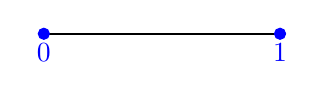
\begin{tikzpicture}
            % Draw the line segment from 0 to 1
            \draw[thick] (0,0) -- (3,0);
            
            % Draw blue endpoints
            \filldraw[blue] (0,0) circle (2pt) node[below] {0};
            \filldraw[blue] (3,0) circle (2pt) node[below] {1};
          \end{tikzpicture}
          \caption{Unit interval $[0, 1]$}
          \label{fig:unit-interval}
        \end{subfigure}
        \hfill 
        \begin{subfigure}[b]{0.48\textwidth}
          \centering
          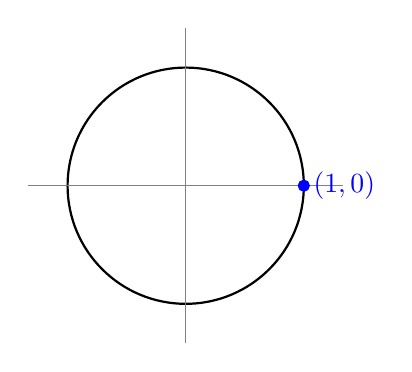
\begin{tikzpicture}
            % Draw the unit circle
            \draw[thick] (0,0) circle (1.5);
            
            % Draw axes for reference
            \draw[gray, thin] (-2,0) -- (2,0);
            \draw[gray, thin] (0,-2) -- (0,2);
            
            % Mark the point (1,0) in blue
            \filldraw[blue] (1.5,0) circle (2pt) node[right] {$(1,0)$};
          \end{tikzpicture}
          \caption{Unit circle $S^1$ in $\mathbb{R}^2$}
          \label{fig:unit-circle}
        \end{subfigure}
        \caption{Visual of the homeomorphism between $[0, 1]$ and $S^1$.}
        \label{fig:comparison}
      \end{figure}

      So can I come up with a function $f: [0, 1] \rightarrow S^1$ s.t. $f(0) = f(1)$? Yes, we can define 
      \begin{equation}
        \bar{f}(x) = (\cos{2 \pi x}, \sin{2\pi x})
      \end{equation}
      Note that we could just chosen $\mathbb{R}^2$ and restricted the image to $S^1$ at the end as well. Therefore, by the theorem above, $X/\sim \cong S^1$, defined by the homeomorphism $\bar{f}(x) = (\cos{2 \pi x}, \sin{2\pi x})$.  
    \end{example}

    \begin{example}[Alternative Construction of 1-Sphere]
      We will show that
      \begin{equation}
        \frac{\mathbb{R}}{\mathbb{Z}} \cong S^1
      \end{equation}
      Let us construct the set $(\mathbb{R}, \T_{\mathbb{R}})$ with paramater $t$. We define maps
      \begin{align*}
        p: \mathbb{R} \rightarrow \mathbb{R} / \mathbb{Z}, \;\; p(t) \equiv t \; (\text{mod } 1) \\
        q: \mathbb[R] \rightarrow S^1 \subset \mathbb{C}, \;\; g(t) \equiv e^{2 \pi i t} 
      \end{align*}
      We claim that $p$ and $q$ are both quotient mappings. Clearly, $p$ is a quotient mapping. As for $q$, it it easy to see that it is surjective (but not injective) and continuous ($\T_{S^1}$ has the basis of open intervals on $S^1$). It is also easy to notice that given an open interval $U \subset S^1$, $q^{-1}(U)$ will be the union of open intervals equally spaced in $\mathbb{R}$. Additionally, given any open interval in $\mathbb{R}$, it maps to an open interval in $S^1$ (note that $S^1$ itself is also open). These three conditions imply that $q$ is a quotient map. We now define maps 
      \begin{align}
        q \circ p^{-1}: & \mathbb{R} / \mathbb{Z} \rightarrow S^1 \\
        p \circ q^{-1}: & S^1 \rightarrow \mathbb{R} / \mathbb{Z}
      \end{align}
      and claim that these maps are homeomorphisms. We can clearly see that the mapping from an open set in $\mathbb{R} / \mathbb{Z}$ to the union of spaced open intervals in $\mathbb{R}$ is an injection, and the mapping from this union of open intervals to the union of open intervals in $S^1$ is a surjection. The composition of these two mappings clearly defines a bijection. Therefore, $q \circ p^{-1}$ is proven to be a bicontinuous bijective mapping between open sets $U \subset \mathbb{R} / \mathbb{Z}$ and $V \subset S^1 \implies$ $q \circ p^{-1}$ is a homeomorphism. 

      This result clearly makes sense since 
      \begin{equation}
        \frac{\mathbb{R}}{\mathbb{Z}} \cong \frac{[0,1]}{\sim}
      \end{equation}
      where the relation $\sim$ maps every point $x \in (0,1)$ to its own equivalence class and the points $0, 1$ to one equivalence class $\{0\}$. Therefore, it is informally said that the quotient space of the real line is a circle. 

      One may attempt to construct a simpler set by replacing $S^1$ with the half-open interval $[0,1)$. However, while $[0,1)$ is bijective to $\mathbb{R} / \mathbb{Z}$,
      \begin{equation}
        \frac{\mathbb{R}}{\mathbb{Z}} \not\cong [0,1)
      \end{equation}
      That is, the two sets are not homeomorphic because the topologies of $[0,1)$ and $\mathbb{R} / \mathbb{Z}$ are not compatible. For instance, when we attempt to map the open set 
      \begin{equation}
        \bigg\{ [x] \in \mathbb{R} / \mathbb{Z} \mid 0 \leq x \leq \frac{1}{4} \vee x > \frac{1}{2} \bigg\} \in \T_{\mathbb{R} / \mathbb{Z}}
      \end{equation}
      to $\T_{[0,1)}$, it does not return an open set. 

      Furthermore, this means that
      \begin{equation}
        S^1 \times S^1 \cong \frac{[0,1]^2}{\sim^\prime} \cong \bigg( \frac{\mathbb{R}}{\mathbb{Z}} \bigg)^2
      \end{equation}
      where $\sim^\prime$ is the quotient mapping defined in the previous construction of the torus. 
    \end{example}

    \begin{example}[Annulus]
      We can construct an annulus with the homeomorphism 
      \begin{equation}
        (x, y) \mapsto \big( (1 + y) \cos{2 \pi x}, (1 + y) \sin{2 \pi x} \big) \in \mathbb{R}^2
      \end{equation}

      \begin{figure}[H]
        \centering
        \begin{subfigure}[b]{0.48\textwidth}
          \centering
          \begin{tikzpicture}
            % Draw square
            \draw (0,0) rectangle (2,2);
            
            % Label top and bottom with >
            \node at (1,2) {$>$};
            \node at (1,-0) {$>$};
          \end{tikzpicture}
          \caption{Unit square $[0,1] \times [0,1]$}
          \label{fig:unit-square}
        \end{subfigure}
        \hfill 
        \begin{subfigure}[b]{0.48\textwidth}
          \centering
          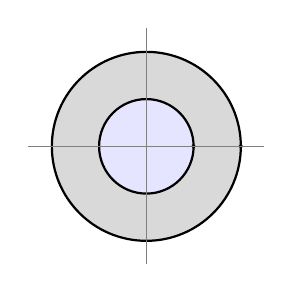
\begin{tikzpicture}[scale=0.6]
            % Fill the annular region with grey (using even-odd rule to keep the inner circle empty)
            \begin{scope}
              \clip (0,0) circle (2);
              \fill[gray!30] (0,0) circle (2);
              \fill[blue!10] (0,0) circle (1);
            \end{scope}
            
            % Draw the two circles
            \draw[thick] (0,0) circle (1);   % Unit circle
            \draw[thick] (0,0) circle (2);   % Circle of radius 2
            
            % Label only the points (1,0) and (2,0)
            \filldraw[font=\footnotesize] (1,0) circle (1pt) node[below] {};
            \filldraw[font=\footnotesize] (2,0) circle (1pt) node[below] {};

            \draw[gray, thin] (-2.5,0) -- (2.5,0);
            \draw[gray, thin] (0,-2.5) -- (0,2.5);
          \end{tikzpicture}
          \caption{Annular region between circles of radius 1 and 2}
          \label{fig:annular-region}
        \end{subfigure}
        \caption{Unit square and annular region}
        \label{fig:annular_comparison}
      \end{figure}
    \end{example}

    \begin{example}[Cylinder]
      Given the unique square $[0, 1]^2$, we can define the equivalence map as $(0, y) \sim (1, y)$ for $y \in [0, 1]$. We claim that this is homeomorphic to the cylinder 
      \begin{equation}
        C \equiv \{(x, y, z) \in \mathbb{R}^3 \mid x^2 + y^2 = 1, z \in [0,1]\} 
      \end{equation}
      with the homeomorphism 
      \begin{equation}
        (x, y) \mapsto \big( \cos{2\pi x}, \sin{2 \pi x}, y \big)
      \end{equation}

      \begin{figure}[H]
        \centering
        \begin{subfigure}[b]{0.48\textwidth}
          \centering
          \begin{tikzpicture}
            % Draw square
            \draw (0,0) rectangle (2,2);
            
            % Label top and bottom with >
            \node at (1,2) {$>$};
            \node at (1,-0) {$>$};
          \end{tikzpicture}
          \caption{Cylinder as an equivalence class on $[0, 1]^2$.}
          \label{fig:cylinder_equiv}
        \end{subfigure}
        \hfill 
        \begin{subfigure}[b]{0.48\textwidth}
          \centering
          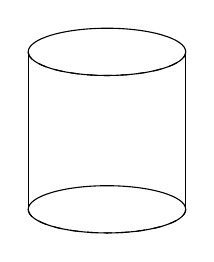
\begin{tikzpicture}
            % Draw cylinder
            \draw (0,0) ellipse (1 and 0.3);
            \draw (0,2) ellipse (1 and 0.3);
            \draw (-1,0) -- (-1,2);
            \draw (1,0) -- (1,2);
            
            % Draw dashed lines to show back of cylinder
            \draw[dashed] (-1,0) arc (180:360:1 and 0.3);
            \draw[dashed] (-1,2) arc (180:360:1 and 0.3);
          \end{tikzpicture}
          \caption{Cylinder as an embedding in $\mathbb{R}^2$. }
          \label{fig:cylinder_embed}
        \end{subfigure}
        \caption{Two geometric figures: a square with labeled sides and a cylinder}
        \label{fig:cylinder}
      \end{figure}
    \end{example}

    \begin{example}[Torus]
      Let $X \equiv [0,1] \times [0,1] \subset \mathbb{R}^2$. We define an equivalence relation $Y$ consisting of the equivalence classes
      \begin{align*}
          &\big\{\{(x, y)\} \mid 0<x, y<1\big\} \cup \big\{ \{(x, 0), (x,1)\} \mid 0<x<1 \big\} \cup \\
          &\big\{ \{(0,y), (1,y)\} \mid 0<y<1 \big\} \cup \big\{ \{(0,0), (0,1), (1,0), (1,1)\} \big\}
      \end{align*} 

      \begin{figure}[H]
        \centering 
        \begin{tikzpicture}
          \draw (0,0) rectangle (2,2);
          \draw (3,0) rectangle (5,2);
          \draw (6,0) rectangle (8,2);
          \draw (9,0) rectangle (11,2);
          \draw[dashed] (1, 1.5) circle [radius=0.4];
          \draw[fill] (1, 1.5) circle [radius=0.03];
          \draw[dashed] (3.9,0) arc (0:180: 0.4);
          \draw[dashed] (3.9,2) arc (0:-180:0.4);
          \draw[dashed] (6,1.1) arc (-90:90:0.4);
          \draw[dashed] (8,1.9) arc (90:270:0.4);
          \draw[fill] (3.5,0) circle [radius=0.03];
          \draw[fill] (3.5,2) circle [radius=0.03];
          \draw[fill] (6,1.5) circle [radius=0.03];
          \draw[fill] (8,1.5) circle [radius=0.03];
          \draw[fill] (9,0) circle [radius=0.03];
          \draw[fill] (11,0) circle [radius=0.03];
          \draw[fill] (9,2) circle [radius=0.03];
          \draw[fill] (11,2) circle [radius=0.03];
          \draw[dashed] (9.4,0) arc (0:90:0.4);
          \draw[dashed] (9.4,2) arc (0:-90:0.4);
          \draw[dashed] (11,0.4) arc (90:180:0.4);
          \draw[dashed] (10.6,2) arc (180:270:0.4);
        \end{tikzpicture}
        \caption{The quotient topology of this quotient space consists of open sets of form. } 
        \label{fig:torus_basis}
      \end{figure}
      This quotient space $X / Y$ is homeomorphic to the torus $S^1 \times S^1$, denoted
      \begin{equation}
        \frac{X}{Y} \cong S^1 \times S^1
      \end{equation}
      We can visualize the construction of the equivalence relation $Y$ as a "gluing" of the rectangle $X$ by its edges and corners. 

      \begin{figure}[H]
        \centering
        \begin{subfigure}[b]{0.48\textwidth}
          \centering
          \begin{tikzpicture}
            % Draw square
            \draw (0,0) rectangle (2,2);
            
            % Label top and bottom with >
            \node at (1,2) {$>$};
            \node at (1,0) {$>$};
            
            % Add >> labels to left and right sides, rotated to point upward
            \node[rotate=90] at (0,1) {$>>$};
            \node[rotate=90] at (2,1) {$>>$};
          \end{tikzpicture}
          \caption{Square with top and bottom sides labeled with $>$}
          \label{fig:square_torus}
        \end{subfigure}
        \hfill 
        \begin{subfigure}[b]{0.48\textwidth}
          \centering
          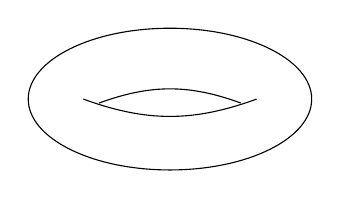
\begin{tikzpicture}
            % Draw torus similar to the reference image
            % Outer ellipse (complete)
            \draw (0,0) ellipse (1.8 and 0.9);
            
            % Inner curves (representing the hole)
            \draw (-0.9, -0.05) to[out=20,in=-200] (0.9, -0.05);
            \draw (-1.1, 0) to[out=-20,in=200] (1.1, 0);
          \end{tikzpicture}
          \caption{Torus}
          \label{fig:torus}
        \end{subfigure}
        \caption{Two geometric figures: a square with labeled sides and a torus}
        \label{fig:geometric-figures}
      \end{figure}
      
      We can check that this mapping is indeed a quotient map. First, it is clearly surjective. By realizing that individual points on the edge of $[0,1]^2$ are open sets themselves (by the subspace topology), we can prove that this map is indeed open and continuous. 
    \end{example}

    \begin{example}[Mobius Strip]
      We can construct the Mobius strip on $[0, 1]^2$ with the equivalence class $(0, y) \sim (1, 1 - y)$ for $y \in [0, 1]$. An explicit parameterization is quite tedious, but we can write the embedding $M \rightarrow \mathbb{R}^3$ with cylindrical coordinates. 
      \begin{figure}[H]
        \centering
        \begin{subfigure}[b]{0.48\textwidth}
          \centering
          \begin{tikzpicture}
            % Draw square
            \draw (0,0) rectangle (2,2);
            
            % Label top and bottom with >
            \node at (1,2) {$>$};
            \node at (1,-0) {$<$};
          \end{tikzpicture}
          \caption{Cylinder as an equivalence class on $[0, 1]^2$.}
          \label{fig:mobius_equiv}
        \end{subfigure}
        \hfill 
        \begin{subfigure}[b]{0.48\textwidth}
          \centering 
          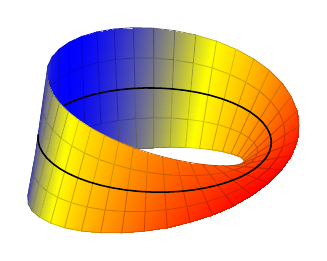
\begin{tikzpicture}[scale=0.7]
            \begin{axis}[
                hide axis,
                view={40}{40}
            ]
            \addplot3 [
                surf, shader=faceted interp,
                point meta=x,
                samples=40,
                samples y=5,
                z buffer=sort,
                domain=0:360,
                y domain=-0.5:0.5
            ] (
                {(1+0.5*y*cos(x/2)))*cos(x)},
                {(1+0.5*y*cos(x/2)))*sin(x)},
                {0.5*y*sin(x/2)});

            \addplot3 [
                samples=50,
                domain=-145:180, % The domain needs to be adjusted manually, depending on the camera angle, unfortunately
                samples y=0,
                thick
            ] (
                {cos(x)},
                {sin(x)},
                {0});
            \end{axis}
          \end{tikzpicture} 
          \caption{Mobius strip has 1 side and is a non-orientable surface.} 
          \label{fig:mobius_strip_r3}
        \end{subfigure}
        \caption{Two geometric figures: a square with labeled sides and a cylinder}
        \label{fig:mobius_strip}
      \end{figure}
    \end{example}

    \begin{example}[2-Sphere]
      Let $X$ be the closed unit ball 
      \begin{equation}
        X \equiv \{(x, y) \in \mathbb{R}^2 \mid x^2 + y^2 \leq 1\}
      \end{equation}
      and define the equialence classes $R$ as 
      \begin{equation}
        R \equiv \big\{ \{(x, y)\} \mid x^2 + y^2 <1 \big\} \cup \{S^1\}
      \end{equation}
      which will consist of open sets of one of the two forms
      \begin{center}
      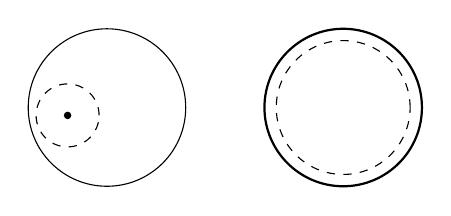
\begin{tikzpicture}
        \draw (1,1) circle [radius=1];
        \draw[thick] (4,1) circle [radius=1];
        \draw[dashed] (0.5,0.9) circle [radius=0.4];
        \draw[fill] (0.5,0.9) circle [radius=0.04];
        \draw[dashed] (4,1) circle [radius=0.85];
      \end{tikzpicture}
      \end{center}
      Then, this quotient space $X / R$ is homeomorphic to the 2-sphere
      \begin{equation}
        S^2 \equiv \{(x, y, z) \in \mathbb{R}^3 \mid x^2 + y^2 + z^2 = 1\}
      \end{equation}
      Visually, we can imagine the disk being glued together by its sides to continuously form the 2-sphere. 
    \end{example}

    \begin{example}[Weird Quotient Space]
      Given $(\mathbb{R}, \T_{\mathbb{R}})$, let us define the relation $\sim$ determined by the quotient mapping 
      \begin{equation}
        p(x) \equiv \begin{cases} \{x\} & x \not\in \mathbb{Z} \\ \mathbb{Z} & x \in \mathbb{Z} \end{cases}
      \end{equation}
      In words, this quotient map maps every integer to the equivalence class $[0]$ and maps every other point to its own class. 

      \begin{figure}[H]
        \centering 
        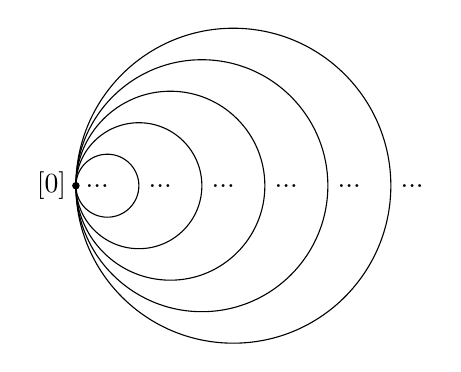
\begin{tikzpicture}[scale=0.4]
          \draw (5,0) circle (5);
          \node[left] at (0,0) {$[0]$};
          \draw[fill] (0,0) circle (0.1);
          \draw (4,0) circle (4);
          \draw (3,0) circle (3);
          \draw (2,0) circle (2);
          \draw (1,0) circle (1);
          \node[right] at (0,0) {...};
          \node[right] at (2,0) {...};
          \node[right] at (4,0) {...};
          \node[right] at (6,0) {...};
          \node[right] at (8,0) {...};
          \node[right] at (10,0) {...};
        \end{tikzpicture}
        \caption{It turns out that every interval $[j, j+1] \subset \mathbb{R}, \; j \in \mathbb{Z}$ will get mapped as a closed loop in $\mathbb{R} / \sim$ beginning and ending with $[0]$, since $j, j+1 \mapsto [0]$. So geometrically, $\mathbb{R} / \sim$ consists of an infinite number of nonintersecting closed loops starting and ending with $[0]$. }
        \label{fig:integer}
      \end{figure}

      This wacky mapping is an example of a quotient mapping that does not preserve topological structure. While it will not be proven here, it is known that $(\mathbb{R}, \T_{\mathbb{R}})$ is 1st and 2nd countable, but $\mathbb{R} / \sim$ under this relation is not even 1st countable. 
    \end{example} 

    Great, so we've went over the construction of quotient topologies and have identified them with some familiar spaces. We end this section with a warning. It was the case that a lot of the properties get passed down to subspaces, but this is not the case for quotient maps. 

    \begin{example}
      Let $X = \mathbb{R}$ with $x \sim y \iff x - y \in \mathbb{Q}$. We claim that $X/\sim$ is uncountable. If we wish to find open sets in $X/\sim$, we can do this by finding saturated open sets in $X$. Let $U \subset \mathbb{R}$ be open and saturated. Since it is open, by the density of $\mathbb{Q}$ in $\mathbb{R}$, $U$ must contain a rational number $\implies \mathbb{Q} \subset U$, and so $U = \mathbb{R}$. Therefore the only saturated open sets are $\emptyset, \mathbb{R}$, meaning that $X/\sim$ has the trivial topology. 
    \end{example}

    This has a lot of consequences, and even very mild topological properties can be broken in quotient spaces.  

    \begin{example}[Quotient of Hausdorff Space Need not be Hausdorff]
      Given $X = \mathbb{R}^2 \setminus \{0\}$ with the ER defined $(x, y) \sim (x^\prime, y^\prime)$ iff $x = x^\prime$, and if $x = x^\prime = 0$, then $\mathrm{sign}(y) = \mathrm{sign}(y^\prime)$. This is the line with 2 origins with the quotient map 
      \begin{equation}
        f(x, y) = \begin{cases} 
          x \text{ if } x \neq 0 \\
          a \text{ if } x = 0, y > 0 \\ 
          b \text{ if } x = 0, y < 0
        \end{cases}
      \end{equation}
    \end{example}

\subsection{Exercises}

  \begin{exercise}[Munkres 16.1]
    Show that if Y is a subspace of X, and A is a subset of Y, then the topology A inherits as a subspace of Y is the same as the topology it inherits as a subspace of X.
  \end{exercise}
  \begin{solution}[Munkres 16.1]
    We have $A \subset (Y, \T_Y) \subset (X, \T_X)$, with $\T_Y$ the subspace topology from $\T_X$. Let us denote $\T_{A|Y}$ and $\T_{A|X}$ the subspace topologies on $A$ when considered its superset as $Y$ and $X$, respectively. We show the following. 
    \begin{enumerate}
      \item $\T_{A|Y} \subset \T_{A|X}$. Let $U \in \T_{A|Y}$. Then $U = V \cap A$ for some $V \in \T_Y$, and $V = W \cap Y$ for some $W \in \T_X$. Therefore, $U = (W \cap Y) \cap A = W \cap (Y \cap A) = W \cap A$ for some $W \in \T_X$, which by definition means $U \in \T_{A|X}$. 
      \item $\T_{A|X} \subset \T_{A|Y}$. Let $U \in \T_{A|X}$. Then $U = V \cap A$ for some $V \in \T_X$. But note that $A = A \cap Y$, and so $U = V \cap (A \cap Y) = (V \cap Y) \cap A$. Denote $W = V \cap Y$. Since $V$ is open in $X$, $W$ is open in $Y$, and therefore we have found such a $W \in \T_Y$ where $U = W \cap A$, which by definition means $U \in \T_{A|Y}$. 
    \end{enumerate}
  \end{solution}

  \begin{exercise}[Munkres 16.2]
    If $\mathcal{T}$ and $\mathcal{T}'$ are topologies on $X$ and $\mathcal{T}'$ is strictly finer than $\mathcal{T}$, what can you say about the corresponding subspace topologies on the subset $Y$ of $X$?
  \end{exercise}

  \begin{exercise}[Munkres 16.3]
    Consider the set Y = [-1, 1] as a subspace of $\mathbb{R}$. Which of the following sets are open in Y? Which are open in $\mathbb{R}$?
    \begin{align}
      A & = \{x \mid \frac{1}{2} < |x| < 1\} \\
      B & = \{x \mid \frac{1}{2} < |x| \leq 1\} \\
      C & = \{x \mid \frac{1}{2} \leq |x| < 1\} \\
      D & = \{x \mid \frac{1}{2} \leq |x| \leq 1\} \\
      E & = \{x \mid 0 < |x| < 1 \text{ and } \frac{1}{x} \notin \mathbb{Z}_+\}
    \end{align}
  \end{exercise}
  \begin{solution}[Munkres 16.3]
    We list the supersets which each set is open in. 
    \begin{enumerate}
      \item A is open in $Y$ and $\mathbb{R}$. $A_1 = (-1, -\frac{1}{2})$ and $A_2 = (\frac{1}{2}, 1)$ are open in $\mathbb{R}$, and they are also open in $Y$ since $A_1 = A_1 \cap Y$ and $A_2 = A_2 \cap Y$. Therefore, $A = A_1 \cup A_2$ is by definition open. 

      \item B is open in $Y$. $(-2, -\frac{1}{2})$ and $(\frac{1}{2}, 2)$ are open in $\mathbb{R}$ and so $(-2, -\frac{1}{2}) \cap Y = [-1, -\frac{1}{2})$ and $(\frac{1}{2}, 2) \cap Y = (\frac{1}{2}, 1]$ is open in $Y$. It is not open in $\mathbb{R}$ because consider the point $1$. Assume that there exists an $\epsilon > 0$ s.t. $(1 - \epsilon, 1 + \epsilon) \subset B$. This means that $1 + \frac{\epsilon}{2} \in (1 - \epsilon, 1 + \epsilon)$ but since $1 < 1 + \frac{\epsilon}{2}$, $1 + \epsilon \not\in B$. 

      \item C. Neither. Consider the point $x = \frac{1}{2}$ and assume that there exists a $\epsilon > 0$ s.t. $B(x, \epsilon) = (\frac{1}{2} - \epsilon, \frac{1}{2} + \epsilon) \subset C$. If $\epsilon > \frac{1}{2}$, then $0 \in B(x, \epsilon)$ and so $B(x, \epsilon) \not\subset C$. If $0 < \epsilon \leq \frac{1}{2}$, then this means that $\frac{1}{2} - \frac{\epsilon}{2} \in B(x, \epsilon)$. But $0 \leq \frac{1}{2} - \frac{\epsilon}{2} < \frac{1}{2}$, and so $\frac{1}{2} - \frac{\epsilon}{2} \not\in C$, which also implies $B(x, \epsilon) \not\subset C$. Therefore there exists no such open neighborhood around $\frac{1}{2}$. This argument applies to both $Y$ and $\mathbb{R}$, and so $C$ is not open in both. 

      \item D. Neither. We repeat the same argument as that for $C$ and show that there exists no open neighborhood around $1/2$ contained in $D$. 

      \item E is open in $Y$ and $\mathbb{R}$. We prove a small fact: for every $x \in \mathbb{R}$, there exists an integer $z \in \mathbb{Z}$ s.t. $z - 1 < x \leq z$. Let's take $x > 0$. The reals is Archimedean and so for any $x \in \mathbb{R}$ there exists a natural $s \in \mathbb{N}$ s.t. $x < n$. Consider the set $N = \{n \in \mathbb{Z} \mid x < n\}$ of all upper bounds of $x$, which we proved is nonempty. By the well-ordering principle, this set must have a minimum, which we call $z$. It must be the case by upper bound that $x \leq z$, and $z-1$ not an upper bound implies $z-1 < x$. If $x = 0$ this result is trivial and if $x < 0$ we can found the integral bounds $0 \leq z - 1 < -x < z$ and swap the signs to get $-z < x < -z + 1 \leq 0$. 

      We claim that 
      \begin{equation}
        G = \{ x \in \mathbb{R} \mid 1/x \not\in \mathbb{N} \} = (-\infty, 0) \cup \bigcup_{n \in \mathbb{N}} \bigg( \frac{1}{n+1}, \frac{1}{n} \bigg) = H
      \end{equation} 
      If $x \in G$, then it can be either positive or negative. If negative, $x \in (-\infty, 0)$. If positive, then $1/x \in \mathbb{R}$ since it's a field. By the proof above there exists a $n \in \mathbb{N}$ s.t. $n < 1/x < n+1$ (strict inequality since $1/x$ is not natural) and so by ordered field properties $\frac{1}{n} < x < \frac{1}{n+1} \implies z \in \big( \frac{1}{n+1}, \frac{1}{n} \big)$ for some $n \in \mathbb{N}$. Therefore $x \in H$. 

      If $x \in H$, then either $x$ is negative or positive. If $x \in (-\infty, 0)$, then $x \in G$ trivially since it cannot be the case that $1/x > 0$. If $x$ is positive then $x \neq 1/n$ for all $n \in \mathbb{N}$, so $x \in G$. Therefore $H = G$. 

      $G$ is an arbitrary union of known open sets in $\mathbb{R}$, and so $G$ is open. This means that $E = ((-1, 0) \cup (0, 1)) \cap H$ is also open by definition, and so $E$ is open in $\mathbb{R}$. For $Y$, note that 
      \begin{equation}
        ((-1, 0) \cup (0, 1)) \cap Y = (-1, 0) \cup (0, 1)
      \end{equation}
      and so $E = E \cap Y$, which implies that $E$ is open in $Y$ as well. 
    \end{enumerate}
  \end{solution}

  \begin{exercise}[Munkres 16.4]
    A map f : X → Y is said to be an open map if for every open set U of X, the set f(U) is open in Y. Show that $\pi_1 : X \times Y \to X$ and $\pi_2 : X \times Y \to Y$ are open maps.
  \end{exercise}
  \begin{solution}[Munkres 16.4] 
    Let $U$ be open in $X \times Y$. Then $U$ is a union of some basis elements of the product topology on $X \times Y$, which are of the form $U_X \times U_Y$ where $U_X, U_Y$ are open sets in the topologies of $X, Y$. 
    \begin{equation}
      U = \bigcup_{\alpha \in A} (U_X)_\alpha  \times (U_Y)_\alpha
    \end{equation} 
    \begin{enumerate}
      \item We see that $\pi_1$ maps all $(x, y) \in U_X \times U_Y$ to $x$, so it acts on $U$ as 
      \begin{equation}
        \pi_1(U) = \bigcup_{\alpha \in A} (U_X)_\alpha
      \end{equation} 
      Since the union of open sets are open, $\pi_1 (U)$ is open in $X$. 

      \item We see that $\pi_2$ maps all $(x, y) \in U_X \times U_Y$ to $y$, so it acts on $U$ as 
      \begin{equation}
        \pi_2(U) = \bigcup_{\alpha \in A} (U_Y)_\alpha
      \end{equation} 
      Since the union of open sets are open, $\pi_2 (U)$ is open in $Y$. 
    \end{enumerate}
  \end{solution}

  \begin{exercise}[Munkres 16.5]
    Let X and X' denote a single set in the topologies $\mathcal{T}$ and $\mathcal{T}'$, respectively; let Y and Y' denote a single set in the topologies $\mathcal{U}$ and $\mathcal{U}'$, respectively. Assume these sets are nonempty.
    \begin{enumerate}
      \item Show that if $\mathcal{T}' \supseteq \mathcal{T}$ and $\mathcal{U}' \supseteq \mathcal{U}$, then the product topology on X' × Y' is finer than the product topology on X × Y.
      \item Does the converse of (a) hold? Justify your answer.
    \end{enumerate}
  \end{exercise}
  \begin{solution}[Munkres 16.5.a] 
    Let us denote the set as $(X,\T), (X, \T^\prime)$ and $(Y, \U), (Y, \U^\prime)$ where $\T \subset \T^\prime$ and $\U \subset \U^\prime$. We wish to show that $\T_{X \times Y} \subset \T_{X^\prime \times X^\prime}$. By Munkres Lemma 13.3, this is equivalent to showing that for any $(x, y) \in X \times Y$ and basis element $U_X \times U_Y \in \T \times \U$ containing $(x, y)$, there is a basis element $U_{X^\prime} \times U_{Y^\prime} \in \T^\prime \times \U^\prime$ such that 
    \begin{equation}
      x \in (U_{X^\prime} \times U_{Y^\prime}) \subset (U_X \times U_Y)
    \end{equation}
    Say we have $(x, y) \in X \times Y$, and choose such a $U_X, U_Y$ containing $x, y$ respectively.\footnote{This is always possible since $X \in \T$ and $Y \in \U$. } Then $U_X \times U_Y \in \T \times \U$ is a basis element of $\T_{X \times Y}$ by definition. We see that $U_X \in \T \subset \T^\prime$ and $U_Y \in \U \subset \U^\prime$, so $U_X \times U_Y \in \T^\prime \times \U^\prime$, meaning that it is also a basis element of $\T_{X^\prime \times Y^\prime}$. Therefore, we set $U_{X^\prime} = U_X$ and $U_{Y^\prime} = U_Y$, and we are done. 
  \end{solution}
  \begin{solution}[Munkres 16.5.b]
    Yes, the converse is true. Let us denote the set as $(X,\T), (X, \T^\prime)$ and $(Y, \U), (Y, \U^\prime)$ where $\T_{X \times Y} \subset \T_{X^\prime \times Y^\prime}$. We wish to show that $\T \subset \T^\prime$ and $\U \subset \U^\prime$. By Munkres Lemma 13.3, it suffices to show that for any $x \in X$ and basis element $B_X \in \T$, there exists a basis element $B_{X^\prime} \in \T^\prime$ such that 
    \begin{equation}
      x \in B_{X^\prime} \subset B_X
    \end{equation} 
    We construct $B_{X^\prime}$ as such. Given $x \in X$ and basis element $B_X \in \T$, choose any $y \in Y$ to get $(x, y) \in X \times Y$, along with the basis element $B_X \times B_Y \in \T_{X \times Y}$.\footnote{Such a basis element $B_Y$ is guaranteed to exist by definition of a basis.} Since $\T_{X^\prime \times Y^\prime}$ is finer, there exists a basis element $U = U_{X^\prime} \times U_{Y^\prime} \in \T_{X^\prime \times Y^\prime}$, where $U_{X^\prime} \in \T^\prime, U_{Y^\prime} \in \U^\prime$, such that 
    \begin{equation}
      (x, y) \in U_{X^\prime} \times U_{Y^\prime} \subset B_X \times B_Y
    \end{equation} 
    Consider the projection map $\pi_1: X \times Y \rightarrow X$, which we have shown in 16.4 to be open. Therefore, by mapping the three expressions through $\pi_1$, we have $x \in U_{X^\prime} \subset B_X$, where $U_{X^\prime} \in \T^\prime$ and $B_X \in \T$. Since open sets are an arbitrary union of basis elements, there exists a basis element $B_{X^\prime} \subset \T^\prime$ satisfying $x \in B_{X^\prime} \subset U_{X^\prime} \subset B_{X}$, and we are done. 

    Since we have shown that the projection $\pi_2$ is also an open map, we can do the exact same argument by choosing any $x \in X$ and a basis element $B_X$ containing $x$, giving us $\U \subset \U^\prime$. 
  \end{solution}

  \begin{exercise}[Munkres 16.6]
    Show that the countable collection
    \[\{(a,b) \times (c,d) \mid a < b \text{ and } c < d, \text{ and } a,b,c,d \text{ are rational}\}\]
    is a basis for $\mathbb{R}^2$.
  \end{exercise}
  \begin{solution}[Munkres 16.6]
    Let's denote the collection as $\mathcal{C}$. For every open set $U$ and each $x \in U$, we know that there exists a $r > 0$ such that the $L_\infty$-open ball $B_\infty (x, r) \subset U$, since the set of such open balls forms a basis. This in $\mathbb{R}^2$ is denoted 
    \begin{equation}
      (x_1 - r, x_1 + r) \times (x_2 - r, x_2 + r)
    \end{equation}
    By the denseness of $\mathbb{Q}$ in $\mathbb{R}$, we can choose an $a, b, c, d \in \mathbb{Q}$ such that $x_1 - r < a < 0 < b < x_1 + r$ and $x_2 - r < c < 0 < d < x_2 + r$, which immediately satisfies. 
    \begin{equation}
      x \in (a, b) \times (c, d) \subset (x_1 - r, x_1 + r) \times (x_2 - r, x_2 + r) = B_\infty (x, r) \subset U
    \end{equation}
    Therefore, by Munkres Lemma 13.2 $\mathcal{C}$ is a basis for the Euclidean topology. 
  \end{solution}

  \begin{exercise}[Munkres 16.7]
    Let $X$ be an ordered set. If $Y$ is a proper subset of $X$ that is convex in $X$, does it follow that $Y$ is an interval or a ray in $X$?
  \end{exercise}

  \begin{exercise}[Munkres 16.8]
    If L is a straight line in the plane, describe the topology L inherits as a subspace of $\mathbb{R}_\ell \times \mathbb{R}$ and as a subspace of $\mathbb{R}_\ell \times \mathbb{R}_\ell$. In each case it is a familiar topology.
  \end{exercise}
  \begin{solution}[Munkres 16.8]  
    The basis of the product topology on $\mathbb{R}_\ell \times \mathbb{R}$ are all sets of form $[a, b) \times (c, d)$. 
    \begin{enumerate}
      \item If $L$ is vertical, then it is the standard topology. 
      \begin{figure}[H]
        \centering 
        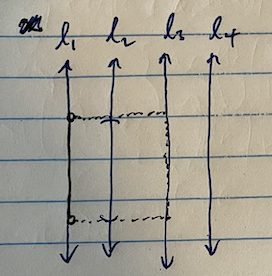
\includegraphics[scale=0.4]{img/1.png}
        \caption{$\ell_1, \ell_2$ intersect the open set at open intervals. $\ell_3, \ell_4$ does not but there are always open sets for which the intersection are open intervals. } 
        \label{fig:1}
      \end{figure}

      \item If $L$ is not vertical, then it is the lower limit topology (or upper limit topology depending on how you parameterize the line). 

      \begin{figure}[H]
        \centering 
        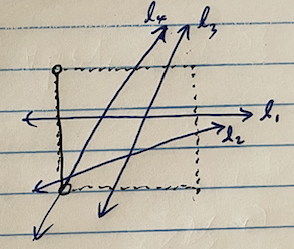
\includegraphics[scale=0.4]{img/2.png}
        \caption{All nonvertical lines will intersect the left ``closed'' side of some open set and will therefore induce the lower/upper limit topology on the line.}
        \label{fig:2}
      \end{figure}
    \end{enumerate}
    The basis of the product topology on $\mathbb{R}_\ell \times \mathbb{R}_\ell$ are all sets of form $[a, b) \times [c, d)$. 
    \begin{enumerate} 
      \item if $L$ has a negative slope (as in the graph represented by $y = mx + b$ where $m < 0$), then it is discrete topology since we can imagine the line intersecting the square at the lower-left corner.\footnote{We can also see it as the topology generated by the basis of closed intervals, but since $[a, b] \cap [b, c] = \{b\}$, this is equivalent to the discrete topology.} 

      \begin{figure}[H]
        \centering 
        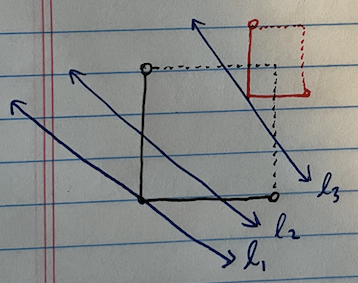
\includegraphics[scale=0.4]{img/3.png}
        \caption{We can construct an open set $[a, b) \times [c, d)$ where the point $(a, c)$ lies on any point on a negatively sloping line. This means that points are open sets, which generates the discrete topology. } 
        \label{fig:3}
      \end{figure}

      \item if $L$ vertical, horizontal, or has a positive slope, then it is the lower limit topology (or upper limit topology depending on how you parameterize the line). 

      \begin{figure}[H]
        \centering 
        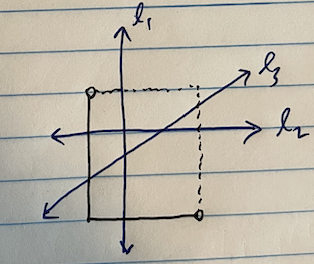
\includegraphics[scale=0.4]{img/4.png}
        \caption{If there is not a negative slope (vertical, horizontal, or positive sloping), then there is no way for a rectangle to intersect the line exactly at the lower-left corner without ``going through'' the rectangle. Therefore these examples generate half-open half-closed intervals on $L$. } 
        \label{fig:4}
      \end{figure}
    \end{enumerate}
  \end{solution}

  \begin{exercise}[Munkres 16.9]
    Show that the dictionary order topology on the set $\mathbb{R} \times \mathbb{R}$ is the same as the product topology $\mathbb{R}_d \times \mathbb{R}$, where $\mathbb{R}_d$ denotes $\mathbb{R}$ in the discrete topology. Compare this topology with the standard topology on $\mathbb{R}^2$.
  \end{exercise}

  \begin{exercise}[Munkres 16.10]
    Let $I = [0, 1]$. Compare the product topology on $I \times I$, the dictionary order topology on $I \times I$, and the topology $I \times I$ inherits as a subspace of $\mathbb{R} \times \mathbb{R}$ in the dictionary order topology.
  \end{exercise}

  \begin{exercise}[Math 411 Spring 2025, PS3]
    Let $P_n$ denote the set of polynomials in n variables with real coefficients. Any such polynomial defines a function on $\mathbb{R}^n$. If A is any subset of $P_n$, let $V(A) = \{x \in \mathbb{R}^n \mid p(x) = 0 \text{ for all } p \in A\}$. A subset $S \subset \mathbb{R}^n$ is called algebraic if it is equal to V(A) for some $A \subset P_n$.

    \begin{enumerate}
      \item Show that $\emptyset$ and $\mathbb{R}^n$ are both algebraic.

      \item Show that if $A_\alpha$ are subsets of $P_n$ (indexed by $\alpha \in I$ for some set I), then
      \[V\left(\bigcup_{\alpha\in I} A_\alpha\right) = \bigcap_{\alpha\in I} V(A_\alpha).\]
      In other words, any intersection of algebraic sets is algebraic.

      \item Suppose $A_1,\ldots,A_k$ are subsets of $P_n$. Let B be the set of polynomials that can be factored as $f = f_1 \cdots f_k$, where $f_i \in A_i$. Prove that
      \[V(B) = V(A_1) \cup \cdots \cup V(A_k).\]
      In other words, any finite union of algebraic sets is algebraic. (Hint: For the inclusion $V(B) \subset V(A_1) \cup \cdots \cup V(A_k)$, it may be easier to show that if $x \not\in V(A_1) \cup \cdots \cup V(A_k)$, then $x \not\in V(B)$.)

      \item Show that $\mathcal{T} = \{U \subset \mathbb{R}^n \mid \mathbb{R}^n - U \text{ is algebraic}\}$ is a topology on $\mathbb{R}^n$. This is known as the Zariski topology, named for the mathematician Oscar Zariski (1899-1986). It is very important in algebraic geometry and related fields.

      \item Show that for n = 1, the Zariski topology on $\mathbb{R}^1$ is precisely the finite complement topology.
    \end{enumerate}

    Note: Instead of doing this with $\mathbb{R}$, you could also do it with $\mathbb{C}$, $\mathbb{Q}$, or any other field.
  \end{exercise}
  \begin{solution}[a]
    Listed. 
    \begin{enumerate}
      \item Consider $A = \{ f(x) = 1\}$. Then $V(A) = \emptyset$ since $f$ never vanishes. 
      \item Consider $A = \{ f(x) = 0 \}$.Then $V(A) = \mathbb{R}^n$ since $f$ always vanishes. 
    \end{enumerate}
  \end{solution}
  \begin{solution}[b]
    We see that 
    \begin{align}
      V \bigg( \bigcup_{\alpha \in I} A_\alpha \bigg) & = \big\{ x \in \mathbb{R}^n \mid \forall p \in \cup_{\alpha \in I} A_\alpha ( p(x) = 0 )\big\} \\ 
                                                      & = \big\{ x \in \mathbb{R}^n \mid \forall \alpha \in I \forall p \in A_\alpha (p(x) = 0)  \big\} \\
                                                      & = \bigcap_{\alpha \in I} \big\{ x \in \mathbb{R}^n \mid \forall p \in A_\alpha (p(x) = 0) \big\} \\
                                                      & = \bigcap_{\alpha \in I} V(A_\alpha)
    \end{align}
  \end{solution}
  \begin{solution}[c]
    We prove bidirectionally. 
    \begin{enumerate}
      \item $\cup_{i} V(A_i) \subset V(B)$. Let $x \in \cup_i V(A_i)$. Then $x \in V(A_j)$ for some $1 \leq j \leq k$, which implies that $f_j (x) = 0$ for all $f_j \in A_j$. Therefore by the field properties of $\mathbb{R}$, 
      \begin{equation}
        f(x) = f_1 (x) \ldots \underbrace{f_j(x)}_{=0} \ldots f_k (x) = 0 
      \end{equation} 
      and therefore $f(x) = 0$ for all $f \in B$, which means that $x \in V(B)$. 

      \item $\cup_i V(A_i) \supset V(B)$. Assume that $x \not\in \cup_i V(A_i)$. Then for all $1 \leq i \leq k$, $x \not\in V(A_i)$, which implies that for all $i$ there exists some $f_i^{\ast} \in A_i$ s.t. $f_i^\ast (x) \neq 0$. Now construct the function $f^\ast = \prod_i f_i^\ast$, where $f_i^\ast \in A_i$, $f^\ast \in B$. But 
      \begin{equation}
        f^\ast (x) = \prod_{i=1}^k f_i^\ast (x) \neq 0
      \end{equation}
      since $f_i^\ast (x) \neq 0$ for all $i$, and so we have shown the existence of a function $f^\ast \in B$ such that $f^\ast (x) \neq 0$. Therefore $x \not\in V(B)$. 
    \end{enumerate}
  \end{solution}
  \begin{solution}[d] 
    We prove the properties of a topology. 
    \begin{enumerate}
      \item From (a), $\emptyset$ is algebraic $\implies \mathbb{R}^n \setminus \emptyset = \mathbb{R}^n$ is in $\mathscr{T}$. Also, $\mathbb{R}^n$ is algebraic $\implies \mathbb{R}^n \setminus \mathbb{R}^n = \emptyset$ is in $\mathscr{T}$.  

      \item Let $\{U_\alpha\}_{\alpha \in I}$ be a collection of open sets in $\mathscr{T}$. Then by definition $\mathbb{R}^n \setminus U_\alpha$ is algebraic, and 
      \begin{equation}
        \mathbb{R}^n \setminus \bigg( \bigcup_{\alpha \in I} U_\alpha \bigg) = \bigcap_{\alpha \in I} (\mathbb{R}^n \setminus U_\alpha) 
      \end{equation} 
      we know from (b) that arbitrary intersections of algebraic sets is algebraic, so the LHS is also algebraic, which by definition means the union is in $\mathscr{T}$. 

      \item Let $U_1, \ldots, U_k$ be a collection of open sets in $\mathscr{T}$. Then by definition $\mathbb{R}^n \setminus U_i$ is algebraic for $1 \leq i \leq k$, and  
      \begin{equation}
        \mathbb{R}^n \setminus \bigg( \bigcap_{i=1}^k U_i \bigg) = \bigcup_{i=1}^k (\mathbb{R}^n \setminus U_i)
      \end{equation}
      we know from (c) that finite unions of algebraic sets is algebraic, and so the LHS is also algebraic, which by definition means the finite intersection is in $\mathscr{T}$. 
    \end{enumerate}
  \end{solution}
  \begin{solution}[e]
    For an open set $U$, inclusion in the finite complement topology asserts that $\mathbb{R} \setminus U$ must be finite or $U = \emptyset$, and inclusion in the Zariski topology asserts that $\mathbb{R} \setminus U$ must be algebraic. Therefore it satisfies to show that the complements (within the universe of the power set) are equal, i.e. that the set of all finite subsets of $\mathbb{R}$ plus $\mathbb{R}$ itself and the set of all algebraic subsets of $\mathbb{R}$ is equal. Let us denote the former $S$ and the latter $T$. 
    \begin{enumerate}
      \item $S \subset T$. Let $Y \in S$ ($Y$ is a set). If $Y = \mathbb{R}$, then it is algebraic as shown in (a). Otherwise, it is finite and we can enumerate it as $Y = \{y_1, \ldots, y_n\}$, and define the singleton subset of polynomials 
      \begin{equation}
        A = \bigg\{ f(x) = \prod_{i=1}^n (x - y_i) \bigg\}
      \end{equation} 
      $V(A)$ consists of all reals where $f(x) = 0$, which happens exactly when $x = y_i$ for some $i$.\footnote{If not, then every $(x - y_i)$ is nonzero, and the product is nonzero.} Therefore, $Y = V(A) \implies Y$ is algebraic $\implies Y \subset T$. 

      \item $T \subset S$. Let $Y \in T$. Then we know that there exists some subset of polynomials $A$ such that $Y = V(A)$. If $A$ is empty, then $V(A) = \mathbb{R}$ since the predicate in the set-builder notation is vacuously true, and $\mathbb{R}$ is contained in the $S$. If $A$ is not empty, then there exists some polynomial $f$ from $A$. By definition it must be the case that for all $y \in Y$, $f(y) = 0$. We consider two cases. 
      \begin{enumerate}
        \item $f$ is constant. If $f \neq 0$, then $V(A) = \emptyset$, which is in $S$. If $f = 0$, then $V(A) = \mathbb{R}$, which is in $S$. 
        \item $f$ has degree $n \geq 1$. Since this is a polynomial ring over a field $\mathbb{F}[x]$, $f(y)$ cannot have more than $n$ real roots.\footnote{Using the single factor theorem of commutative rings we can use induction to prove that the set of roots cannot go beyond $n$. For linear polynomials $f(x) = mx + b$ there is one root $x = -b/m$ which satisfies the base case, and for higher degrees of $n$ we show that if there is a root where $p(a) = 0$, then $p(x) = (x - a) q(x)$ where $q$ is of degree $n-1$ which cannot have more than $n-1$ factors.} Therefore $|Y| \leq n$ and $Y$ must be finite. 
      \end{enumerate}

      We have shown that $V(\{f\})$ is finite. Since $V(A)$ consists of $y$'s that hold for all $f \in A$, $V(A) \subset V(\{f\})$.\footnote{To see why, look at my solution for (b).} The subset of finite sets is finite, and therefore $Y = V(A) \in S$. 
    \end{enumerate}
  \end{solution}

  \begin{exercise}[Munkres 19.4]
    Show that $(X_1 \times \cdots \times X_{n-1}) \times X_n$ is homeomorphic with $X_1 \times \cdots \times X_n$.
  \end{exercise}

  \begin{exercise}[Munkres 19.5]
    One of the implications stated in Theorem 19.6 holds for the box topology. Which one?
  \end{exercise}

  \begin{exercise}[Munkres 19.6]
    Let $\mathbf{x}_1, \mathbf{x}_2, \ldots$ be a sequence of the points of the product space $\prod X_\alpha$. Show that this sequence converges to the point $\mathbf{x}$ if and only if the sequence $\pi_\alpha(\mathbf{x}_1), \pi_\alpha(\mathbf{x}_2), \ldots$ converges to $\pi_\alpha(\mathbf{x})$ for each $\alpha$. Is this fact true if one uses the box topology instead of the product topology?
  \end{exercise}

  \begin{exercise}[Munkres 19.7]
    Let $\mathbb{R}^\infty$ be the subset of $\mathbb{R}^\omega$ consisting of all sequences that are ``eventually zero,'' that is, all sequences $(x_1, x_2, \ldots)$ such that $x_i \neq 0$ for only finitely many values of $i$. What is the closure of $\mathbb{R}^\infty$ in $\mathbb{R}^\omega$ in the box and product topologies? Justify your answer.
  \end{exercise}
  \begin{solution}
    In the box topology, $\overline{\mathbb{R}^\infty} = \mathbb{R}^\infty$. We show this by taking any sequence not in $\mathbb{R}^\infty$ and showing that there exists an open neighborhood that has a trivial intersection with $\mathbb{R}^\infty$. Consider a non-eventually zero sequence $y \in \mathbb{R}^\omega \setminus \mathbb{R}^\infty$, which must have an infinite number of nonzero terms. $y$ is contained within the open set (in the box topology) 
    \begin{equation}
      U = U_1 \times U_2 \times \ldots, \qquad U_i = 
      \begin{cases}
        (0, +\infty) & \text{ if } y_i > 0 \\
        (-1, 1)  & \text{ if } y_i = 0 \\
        (-\infty, 0) & \text{ if } y_i < 0
      \end{cases}
    \end{equation}
    This is an open set that clearly contains $y$, but it has an empty intersection with $\mathbb{R}^\omega$ since there are an infinite number of nonzero terms $y_i$ and so there are an infinite number of $U_i$'s that do not contain $0$. 

    In the product topology, basis elements are all sets of the form $\prod U_i$ where $U_i$ is open in $\mathbb{R}$ and $U_i = \mathbb{R}$ except for finitely many values of $i$. Therefore, $U_i \neq \mathbb{R}$ for finite values. Now given any sequence $y \in \mathbb{R}^\omega$, we claim that it is a limit point of $\mathbb{R}^\infty$. An open neighborhood of $y$ of form $U_y = \prod U_i$ must have some maximum index $N$ for which $U_i = \mathbb{R}$ when $i > N$, and so the eventually-zero sequence $x = (y_1, y_2, \ldots, y_N, 0, 0 ,\ldots)$ must be in $U$, implying that $U_y \cap \mathbb{R}^\infty \neq \emptyset$, and so $y$ is a limit point of $U_y$. Therefore all sequences are limit points, which means $\overline{\mathbb{R}^\infty} = \mathbb{R}^\omega$. 
  \end{solution}

  \begin{exercise}[Munkres 19.8]
    Given sequences $(a_1, a_2, \ldots)$ and $(b_1, b_2, \ldots)$ of real numbers with $a_i > 0$ for all $i$, define $h : \mathbb{R}^\omega \to \mathbb{R}^\omega$ by the equation
    \begin{equation}
      h((x_1, x_2, \ldots)) = (a_1x_1 + b_1, a_2x_2 + b_2, \ldots).
    \end{equation}
    Show that if $\mathbb{R}^\omega$ is given the product topology, $h$ is a homeomorphism of $\mathbb{R}^\omega$ with itself. What happens if $\mathbb{R}^\omega$ is given the box topology?
  \end{exercise}
  \begin{solution}
    We first show $h$ is a bijection. Indeed, the element-wise mappings are bijections and the inverse is 
    \begin{equation}
      h^{-1} ((x_1, \ldots, )) = \bigg(\ldots,  \frac{x_i - b_i}{a_i}, \ldots \bigg)
    \end{equation} 
    Now we show that it is continuous. Given an open set in $\mathbb{R}^\omega$ in the product topology, it has the form 
    \begin{equation}
      U = (l_1, u_1) \times (l_2, u_2) \times \ldots \times (l_n, u_n) \times \mathbb{R} \times \ldots 
    \end{equation} 
    The preimage under $h$ is 
    \begin{equation}
      h^{-1} (U) = \bigg( \frac{l_1 - b_1}{a_1}, \frac{u_1 - b_1}{a_1} \bigg) \times \ldots \times \bigg( \frac{l_n - b_n}{a_n}, \frac{u_n - b_n}{a_n} \bigg) \times \mathbb{R} \times \ldots
    \end{equation}
    where $l_1 < u_1 \implies (l_1 - b_1) /a_1 < (u_1 - b_1) / a_1$. This is also of the form of open sets in the product topology, and therefore is continuous. Now considering the continuity of the inverse function, we can see that taking the same $U$ as before, we have 
    \begin{equation}
      h(U) = (a_1 l_1 + b_1, a_1 u_1 + b_1) \times \ldots \times (a_n l_n + b_n, a_n u_n + b_n) \times \mathbb{R} \ldots 
    \end{equation}
    which is also open in the product topology. Therefore $h$ is a homeomorphism under the product topologies. 

    Now we consider the box topology. Given an box-topology open set of the form 
    \begin{equation}
      U = (l_1, u_1) \times (l_2, u_2) \times \ldots
    \end{equation} 
    then the preimage and image are 
    \begin{align}
      h^{-1} (U) & = \bigg( \frac{l_1 - b_1}{a_1}, \frac{u_1 - b_1}{a_1} \bigg) \times \bigg( \frac{l_2 - b_2}{a_2}, \frac{u_2 - b_2}{a_2} \bigg) \times \ldots \\
      h(U) & = h(U) = (a_1 l_1 + b_1, a_1 u_1 + b_1) \times (a_2 l_2 + b_2, a_2 u_2 + b_2) \times 
    \end{align}
    which are both open in the box topology and so $h$ and $h^{-1}$ are continuous. Thus $h$ is also a homeomorphism. 
  \end{solution}

  \begin{exercise}[Munkres 19.9]
    Show that the choice axiom is equivalent to the statement that for any indexed family $\{A_\alpha\}_{\alpha \in J}$ of nonempty sets, with $J \neq \emptyset$, the cartesian product
    \begin{align*}
      \prod_{\alpha \in J} A_\alpha
    \end{align*}
    is not empty.
  \end{exercise}

  \begin{exercise}[Munkres 19.10]
    Let $A$ be a set; let $\{X_\alpha\}_{\alpha \in J}$ be an indexed family of spaces; and let $\{f_\alpha\}_{\alpha \in J}$ be an indexed family of functions $f_\alpha : A \to X_\alpha$.
    \begin{enumerate}
      \item Show there is a unique coarsest topology $\mathcal{T}$ on $A$ relative to which each of the functions $f_\alpha$ is continuous.
      \item Let
      \begin{align*}
        S_\beta = \{f_\beta^{-1}(U_\beta) \mid U_\beta \text{ is open in } X_\beta\},
      \end{align*}
      and let $S = \bigcup S_\beta$. Show that $S$ is a subbasis for $\mathcal{T}$.
      \item Show that a map $g : Y \to A$ is continuous relative to $\mathcal{T}$ if and only if each map $f_\alpha \circ g$ is continuous.
      \item Let $f : A \to \prod X_\alpha$ be defined by the equation
      \begin{align*}
        f(a) = (f_\alpha(a))_{\alpha \in J};
      \end{align*}
      let $Z$ denote the subspace $f(A)$ of the product space $\prod X_\alpha$. Show that the image under $f$ of each element of $\mathcal{T}$ is an open set of $Z$.
    \end{enumerate}
  \end{exercise}

  \begin{exercise}[Munkres 22.2]
    \begin{enumerate}
      \item[(a)] Let $p : X \to Y$ be a continuous map. Show that if there is a continuous map
        $f : Y \to X$ such that $p \circ f$ equals the identity map of $Y$, then $p$ is a quotient
        map.
      
      \item[(b)] If $A \subset X$, a \textit{retraction} of $X$ onto $A$ is a continuous map $r : X \to A$ such
        that $r(a) = a$ for each $a \in A$. Show that a retraction is a quotient map.
    \end{enumerate}
  \end{exercise}
  \begin{solution}
     Listed. 
     \begin{enumerate}
       \item Let $U \subset Y$, and let $p^{-1}(U)$ be open. Then, 
       \begin{align}
         p^{-1} (U) \subset X \text{ open} & \implies f^{-1} (p^{-1}(U)) \subset Y \text{ open} \\
                                           & \implies (p \circ f)^{-1} (U) = U \subset Y \text{ open}
       \end{align}
       and since $p$ is continuous, $p$ is a quotient map. Since $p \circ f$ equals the identity map, it must be the case that $p$ is surjective. 

       \item We know that the canonical injection $\iota: A \rightarrow X$ is continuous, and $r \circ \iota = I$, the identity map of $A$. Therefore by (a), $p$ is a quotient map. 
     \end{enumerate}
  \end{solution}

  \begin{exercise}[Munkres 22.3]
    Let $\pi_1 : \mathbb{R} \times \mathbb{R} \to \mathbb{R}$ be projection on the first coordinate. Let $A$ be the subspace of $\mathbb{R} \times \mathbb{R}$ consisting of all points $x \times y$ for which either $x \geq 0$ or $y = 0$ (or both); let $q : A \to \mathbb{R}$ be obtained by restricting $\pi_1$. Show that $q$ is a quotient map that is neither open nor closed.
  \end{exercise}
  \begin{solution} 
    The restriction of a continuous function is always continuous, so $q$ is continuous. Furthermore $q$ is surjective since given any $x \in \mathbb{R}$, we can always see that $(x, 0) \in q^{-1}(\{x\})$. Finally, let $U \subset \mathbb{R}$ s.t. $q^{-1} (U) \subset A$ is open. Then, for any $x \in U$, we know $(x, 0) \subset q^{-1} (U)$, and so  $\exists \epsilon > 0$ s.t. $B((x, 0), \epsilon) \cap A) \subset q^{-1} (U)$. Mapping both sides through $q$ again gives 
    \begin{equation}
      (x - \epsilon, x + \epsilon) = q\big( B((x, 0), \epsilon) \cap A) \big) \subset q (q^{-1}(U)) = U
    \end{equation}
    and so $U$ is open. Therefore, $q$ is a quotient map. To see why it is not open, consider the open set of $A$ 
    \begin{equation}
      U = [0, 1) \times (0, 1) = [(-1, 1) \times (0, 1)] \cap A 
    \end{equation} 
    Then $q(U) = [0, 1)$ which is not open in $\mathbb{R}$. To see why not closed, consider the closed set $C = \{(x, y) \in \mathbb{R}^2 \mid xy = 1, x > 0 \}$.\footnote{Also stated to be closed by example 2 of chapter 22.} Then $p(C) = (0, +\infty)$ which is not closed in $\mathbb{R}$. 
  \end{solution}

  \begin{exercise}[Munkres 22.4]
    \begin{enumerate}
      \item[(a)] Define an equivalence relation on the plane $X = \mathbb{R}^2$ as follows:
      \begin{center}
        $x_0 \times y_0 \sim x_1 \times y_1$ \quad if $x_0 + y_0^2 = x_1 + y_1^2$.
      \end{center}
      Let $X^*$ be the corresponding quotient space. It is homeomorphic to a familiar
      space; what is it? 
      
      \item[(b)] Repeat (a) for the equivalence relation
      \begin{center}
        $x_0 \times y_0 \sim x_1 \times y_1$ \quad if $x_0^2 + y_0^2 = x_1^2 + y_1^2$.
      \end{center}
    \end{enumerate}
  \end{exercise}
  \begin{solution}
    Listed. 
    \begin{enumerate}
      \item Graphing this shows that $X^\ast$ is the set of all horizontal parabolas of the same scale and opening leftwards with the vertex on the $x$-axis, i.e. the elements are just left-right shifts of one another. We claim that it is homeomorphic to $\mathbb{R}$. Let $p: \mathbb{R}^2 \rightarrow X^\ast$ be the quotient map and $f: \mathbb{R}^2 \rightarrow \mathbb{R}$ be defined $f(x, y) = x + y^2$, which satisfies $(x,y) \sim (x^\prime, y^\prime) \iff f(x, y) = f(x^\prime, y^\prime)$. Therefore, this induces a function $\bar{f}: X^\ast  \rightarrow \mathbb{R}$ s.t. $\bar{f} \circ p = f$. Since $f$ is continuous, $\bar{f}$ is continuous. Also, we can see that $\bar{f}$ is a bijection since we can map every element in the equivalence class of $[(x, y)]$ s.t. $x + y^2 = c$ to $c \in \mathbb{R}$. Finally, we show that $\bar{f}^{-1}$ is continuous. We can think of $\bar{f}^{-1}$ as the composition of maps $c \mapsto (c, 0) \mapsto [(c, 0)]$, where the first map is trivially continuous and the second map is $p$, which is also continuous. Therefore $\bar{f}^{-1}$ is continuous, and it is a homeomorphism. 
        
      \item We can see that $X^\ast$ is the set of all circles of nonnegative radius (the origin is a circle of radius $0$), and we claim that it is homeomorphic to $[0, +\infty)$. Let $p: \mathbb{R}^2 \rightarrow X^\ast$ be the quotient map and $f: \mathbb{R}^2 \rightarrow [0, +\infty)$ be defined $f(x, y) = x^2 + y^2$, which satisfies $(x,y) \sim (x^\prime, y^\prime) \iff f(x, y) = f(x^\prime, y^\prime)$. Therefore, this induces a function $\bar{f}: X^\ast  \rightarrow [0, +\infty)$ s.t. $\bar{f} \circ p = f$. Since $f$ is continuous, $\bar{f}$ is continuous. Also, we can see that $\bar{f}$ is a bijection since we can map every element in the equivalence class of $[(x, y)]$ s.t. $x^2 + y^2 = c$ to $c \in [0, +\infty)$. Finally, we show that $\bar{f}^{-1}$ is continuous. We can think of $\bar{f}^{-1}$ as the composition of maps $c \mapsto (\sqrt{c}, 0) \mapsto [(\sqrt{c}, 0)]$, where the first map is continuous\footnote{The square root function from $\mathbb{R}_0^+$ to itself is continuous since the preimage of an open interval $(a, b)$ is $(\sqrt{a}, \sqrt{b})$ which is also open in $\mathbb{R}_0^+$, and for $[0, b)$ the preimage is $[0, \sqrt{b})$.} and the second map is $p$, which is also continuous. Therefore $\bar{f}^{-1}$ is continuous, and it is a homeomorphism. 
    \end{enumerate}
  \end{solution}

  \begin{exercise}[Munkres 22.5]
    Let $p : X \to Y$ be an open map. Show that if $A$ is open in $X$, then the map $q : A \to p(A)$ obtained by restricting $p$ is an open map.
  \end{exercise}

  \begin{exercise}[Munkres 22.6]
    Recall that $\mathbb{R}_K$ denotes the real line in the $K$-topology. (See \S13.) Let $Y$ be the quotient space obtained from $\mathbb{R}_K$ by collapsing the set $K$ to a point; let $p : \mathbb{R}_K \to Y$ be the quotient map.
    \begin{enumerate} 
      \item[(a)] Show that $Y$ satisfies the $T_1$ axiom, but is not Hausdorff.
      \item[(b)] Show that $p \times p : \mathbb{R}_K \times \mathbb{R}_K \to Y \times Y$ is not a quotient map. [Hint: The diagonal is not closed in $Y \times Y$, but its inverse image is closed in $\mathbb{R}_K \times \mathbb{R}_K$.]
    \end{enumerate}
  \end{exercise}

  \begin{exercise}[Math 411 Spring 2025, PS6]
    For each integer $n \geq 1$, let us consider the following spaces:
    \begin{align*}
      S^n &= \{\mathbf{x} \in \mathbb{R}^{n+1} \mid \|\mathbf{x}\|= 1\} \\
      X^{n+1} &= \mathbb{R}^{n+1} - \{\mathbf{0}\}
    \end{align*}
    (Note: the superscript is just a decoration that indicates the ``dimensionality''
    of the space; it does \textit{not} indicate raising something to a power.)
    \begin{enumerate}
      \item[(1)] Show that the function $r : X^{n+1} \to S^n$ defined by $r(\mathbf{x}) = \mathbf{x}/\|\mathbf{x}\|$ is a
        quotient map, and describe the corresponding equivalence relation. (Hint:
        Use \#2 from \S22.)
        
      \item[(2)] We now define a space called \textit{real projective n-space}, or $\mathbb{RP}^n$. We can
        define it in either of two ways:
        \begin{enumerate}
          \item[(a)] $X^{n+1}/{\sim}$, where $\mathbf{x} \sim \mathbf{y}$ iff $\mathbf{x} = \lambda\mathbf{y}$ for some $\lambda \in \mathbb{R} - \{0\}$.
          \item[(b)] $S^n/{\sim}$, where $\mathbf{x} \sim \mathbf{y}$ iff $\mathbf{x} = \pm\mathbf{y}$.
        \end{enumerate}
        Let $p : X^{n+1} \to \mathbb{RP}^n$ be the quotient map. Prove that $p|_{S^n} : S^n \to \mathbb{RP}^n$ is
        also a quotient map, and hence that the two descriptions above produce
        homeomorphic spaces. (Hint: It may help to observe that $p|_{S^n} \circ r = p$.)
        
      \item[(3)] Using the description of $\mathbb{RP}^n$ as a quotient of $S^n$, prove that $\mathbb{RP}^n$ is
        a Hausdorff space. (Hint: note that for $\mathbf{x} \in S^n$ and $\epsilon > 0$, the set
        $(B(\mathbf{x},\epsilon) \cup B(-\mathbf{x},\epsilon)) \cap S^n$ is open and saturated.)
        
      \item[(4)] Let $D^n_+$ denote the ``upper hemisphere'' in $S^n$: $D^n_+ = \{\mathbf{x} \in S^n \mid x_{n+1} \geq 0\}$.
        Show that $D^n_+$ is homeomorphic to $D^n = \{\mathbf{x} \in \mathbb{R}^n \mid \|\mathbf{x}\| \leq 1\}$, the unit
        disk in $\mathbb{R}^n$.
        
      \item[(5)] The restriction of $p$ to $D^n$, viewed as a map $D^n \to \mathbb{RP}^n$, can be shown
        to be a quotient map. Assuming this, describe an equivalence relation
        on $D^n$ whose quotient space is homeomorphic to $\mathbb{RP}^n$. In the case where
        $n = 2$, describe how we may concretely describe $\mathbb{RP}^2$ as a ``video game.''
    \end{enumerate}
  \end{exercise}
  \begin{solution}
    Listed. 
    \begin{enumerate}
      \item We claim $r$ is a retraction, since $r(x) = x$ for all $x \in S^n \subset \mathbb{R}^{n+1}$. $r$ is also continuous since a basis element of the topology of $S^n$ can be written $B = \big\{(a_1, b_1) \times \ldots \times (a_{n+1}, b_{n+1}) \big\} \cap S^n$. Therefore the preimage of such a set is 
      \begin{equation}
        r^{-1} (B) = \bigcup_{c > 0} \big\{(c a_1, c b_1) \times \ldots \times (c a_{n+1}, c b_{n+1}) \big\} \cap S^n 
      \end{equation}
      which is the union of open sets in $S^n$ and therefore is open in $S^n$. From the first exercise, $r$ is a quotient map. It consists of each ray starting from the origin, and maps each direction to the unit vector, creating a sphere.   


      \item $p|_{S^n} \circ r = p$. Since $p$ is a quotient map, it is continuous and its restriction $p|_{S^n}$ is also continuous. Since $p$ is a quotient map, it is surjective and therefore $p|_{S^n}$ must be surjective.\footnote{If $p|_{S^n}$ wasn't surjective, then $p|_{S^n} \circ r$ is not surjective and $p$ is not surjective, a contradiction. } Now let $U \subset \mathbb{RP}^n$ s.t. $p|_{S^n}^{-1} (U)$ is open in $S^n$. Then, 
      \begin{equation}
        r^{-1} \big( p|_{S^n}^{-1} (U) \big) = (p |_{S^n} \circ r)^{-1} (U) = p^{-1} (U)
      \end{equation} 
      is open since $r$ is continuous. But since $p$ is a quotient map, $U$ is open, implying that $p|_{S^n}$ is a quotient map. Therefore, we have shown that 
      \begin{equation}
        X^{n+1} / \sim \cong \mathbb{RP}^n \text{ and } S^n / \sim \cong \mathbb{RP}^n \implies X^{n+1} / \sim \cong S^n / \sim
      \end{equation}

      \item Let us have $x, y \in \mathbb{RP}^n$ with $x \neq y$. Then there exists $u, v \in S^n$ s.t. $p|_{S^n}^{-1}(x) = \{u, -u\}$ and $p|_{S^n}^{-1} (y) = \{v, -v\}$. We can let $\epsilon = \frac{1}{2} \min\{ \|u - v\|, \|u + v\|\}$, which means that 
      \begin{equation}
        B(\pm u, \epsilon) \cap B(\pm v, \epsilon) = \emptyset 
      \end{equation}
      in $\mathbb{R}^n$, and so the open neighborhoods around $\pm u, \pm v$, denoted $U_{\pm}, V_{\pm}$ are all pairwise disjoint in $S^n$. Note that $U_+ \cup U_-$ and $V_+ \cup V_-$ are open, saturated, and disjoint, and so $p|_{S^n}$, as a quotient map, maps both of these sets to disjoint open neighborhoods of $x, y$, proving that $\mathbb{RP}^n$ is Hausdorff. 

      \item We can visualize this as if we were just ``pushing up'' the disk onto the hemisphere. More formally, let us define $f: D^n \rightarrow D_+^n$ as 
      \begin{equation}
        f(x) = f(x_1, \ldots, x_n) = (x_1, \ldots, x_n, \sqrt{1 - \|x\|})
      \end{equation}
      This is well-defined since we assume that $\|x\| \leq 1$. This is trivially injective since changing any of the $x_i$'s will result in a different values in the first $n$ terms of the output. It is surjective since given any element $y = (y_1, \ldots, y_{n+1}) \in D_+$, we know that $\|y\| = 1$ and so we can find the preimage to be $x = (y_1, \ldots, y_n)$ which will satisfy $\|x\| \leq 1$. Therefore, $f$ is bijective, with the inverse function 
      \begin{equation}
        f^{-1} (y) = f^{-1} (y_1, \ldots, y_{n+1}) = (y_1, \ldots, y_{n})
      \end{equation}
      To prove continuity of $f$, consider the basis element of the form 
      \begin{equation}
        (a_1, b_1) \times \ldots \times (a_{n+1}, b_{n+1}) \cap D_+^n 
      \end{equation}
      the preimage is 
      \begin{equation}
        f^{-1} \big( (a_1, b_1) \times \ldots \times (a_{n+1}, b_{n+1})\big) \cap f^{-1} (D_+^n) = (a_1, b_1) \times (a_n, b_n) \cap D^n 
      \end{equation}
      which is a basis element of $D^n$. To prove continuity of $f^{-1}$, we consider its extension $f^{-1}: \mathbb{R}^{n+1} \rightarrow \mathbb{R}^n$, which is simply a projection of the first $n$ elements and is therefore continuous. The restriction of this function $f^{-1}: D_+^n \rightarrow \mathbb{R}^n$ is therefore continuous, and since the image of $f^{-1}$ only hits $D^n$, every open set in $D^n$ is of the form $U = V \cap D^n$ for $V$ open in $\mathbb{R}^n$, where the preimage will simply be $f(U) = f(V) \cap f(D^n)$. We know $f(V)$ is open\footnote{by continuity of $f^{-1}$ with codomain $\mathbb{R}^n$} and $f(D^n) = D^n_+$, $f(U)$ is open in $D_+^n$. 

      \item In $D^n$, we define the equivalence relation $\sim$ where $x \sim -x$ if $\|x\| = 1$, and every other point (in the interior of the disk) is equivalent to itself only. When $n=2$, we can imagine a player walking in a circular disk in $\mathbb{R}^2$, and when it crosses the boundary it will end up at the antipodal point. 
    \end{enumerate}
  \end{solution}


